\documentclass[twoside]{book}

% Packages required by doxygen
\usepackage{fixltx2e}
\usepackage{calc}
\usepackage{doxygen}
\usepackage[export]{adjustbox} % also loads graphicx
\usepackage{graphicx}
\usepackage[utf8]{inputenc}
\usepackage{makeidx}
\usepackage{multicol}
\usepackage{multirow}
\PassOptionsToPackage{warn}{textcomp}
\usepackage{textcomp}
\usepackage[nointegrals]{wasysym}
\usepackage[table]{xcolor}

% Font selection
\usepackage[T1]{fontenc}
\usepackage[scaled=.90]{helvet}
\usepackage{courier}
\usepackage{amssymb}
\usepackage{sectsty}
\renewcommand{\familydefault}{\sfdefault}
\allsectionsfont{%
  \fontseries{bc}\selectfont%
  \color{darkgray}%
}
\renewcommand{\DoxyLabelFont}{%
  \fontseries{bc}\selectfont%
  \color{darkgray}%
}
\newcommand{\+}{\discretionary{\mbox{\scriptsize$\hookleftarrow$}}{}{}}

% Page & text layout
\usepackage{geometry}
\geometry{%
  a4paper,%
  top=2.5cm,%
  bottom=2.5cm,%
  left=2.5cm,%
  right=2.5cm%
}
\tolerance=750
\hfuzz=15pt
\hbadness=750
\setlength{\emergencystretch}{15pt}
\setlength{\parindent}{0cm}
\setlength{\parskip}{3ex plus 2ex minus 2ex}
\makeatletter
\renewcommand{\paragraph}{%
  \@startsection{paragraph}{4}{0ex}{-1.0ex}{1.0ex}{%
    \normalfont\normalsize\bfseries\SS@parafont%
  }%
}
\renewcommand{\subparagraph}{%
  \@startsection{subparagraph}{5}{0ex}{-1.0ex}{1.0ex}{%
    \normalfont\normalsize\bfseries\SS@subparafont%
  }%
}
\makeatother

% Headers & footers
\usepackage{fancyhdr}
\pagestyle{fancyplain}
\fancyhead[LE]{\fancyplain{}{\bfseries\thepage}}
\fancyhead[CE]{\fancyplain{}{}}
\fancyhead[RE]{\fancyplain{}{\bfseries\leftmark}}
\fancyhead[LO]{\fancyplain{}{\bfseries\rightmark}}
\fancyhead[CO]{\fancyplain{}{}}
\fancyhead[RO]{\fancyplain{}{\bfseries\thepage}}
\fancyfoot[LE]{\fancyplain{}{}}
\fancyfoot[CE]{\fancyplain{}{}}
\fancyfoot[RE]{\fancyplain{}{\bfseries\scriptsize Generated by Doxygen }}
\fancyfoot[LO]{\fancyplain{}{\bfseries\scriptsize Generated by Doxygen }}
\fancyfoot[CO]{\fancyplain{}{}}
\fancyfoot[RO]{\fancyplain{}{}}
\renewcommand{\footrulewidth}{0.4pt}
\renewcommand{\chaptermark}[1]{%
  \markboth{#1}{}%
}
\renewcommand{\sectionmark}[1]{%
  \markright{\thesection\ #1}%
}

% Indices & bibliography
\usepackage{natbib}
\usepackage[titles]{tocloft}
\setcounter{tocdepth}{3}
\setcounter{secnumdepth}{5}
\makeindex

% Hyperlinks (required, but should be loaded last)
\usepackage{ifpdf}
\ifpdf
  \usepackage[pdftex,pagebackref=true]{hyperref}
\else
  \usepackage[ps2pdf,pagebackref=true]{hyperref}
\fi
\hypersetup{%
  colorlinks=true,%
  linkcolor=blue,%
  citecolor=blue,%
  unicode%
}

% Custom commands
\newcommand{\clearemptydoublepage}{%
  \newpage{\pagestyle{empty}\cleardoublepage}%
}

\usepackage{caption}
\captionsetup{labelsep=space,justification=centering,font={bf},singlelinecheck=off,skip=4pt,position=top}

%===== C O N T E N T S =====

\begin{document}

% Titlepage & ToC
\hypersetup{pageanchor=false,
             bookmarksnumbered=true,
             pdfencoding=unicode
            }
\pagenumbering{roman}
\begin{titlepage}
\vspace*{7cm}
\begin{center}%
{\Large QT Tcp Server \\[1ex]\large 0.\+0.\+1 }\\
\vspace*{1cm}
{\large Generated by Doxygen 1.8.11}\\
\end{center}
\end{titlepage}
\clearemptydoublepage
\tableofcontents
\clearemptydoublepage
\pagenumbering{arabic}
\hypersetup{pageanchor=true}

%--- Begin generated contents ---
\chapter{Namespace Index}
\section{Lista de namespaces}
Lista dos namespaces com uma breve descrição\+:\begin{DoxyCompactList}
\item\contentsline{section}{\hyperlink{namespace_ui}{Ui} }{\pageref{namespace_ui}}{}
\end{DoxyCompactList}

\chapter{Hierarchical Index}
\section{Class Hierarchy}
This inheritance list is sorted roughly, but not completely, alphabetically\+:\begin{DoxyCompactList}
\item Q\+Main\+Window\begin{DoxyCompactList}
\item \contentsline{section}{Main\+Window}{\pageref{class_main_window}}{}
\end{DoxyCompactList}
\end{DoxyCompactList}

\chapter{Class Index}
\section{Lista de componentes}
Lista de classes, estruturas, uniões e interfaces com uma breve descrição\+:\begin{DoxyCompactList}
\item\contentsline{section}{\hyperlink{class_main_window}{Main\+Window} \\*A classe \hyperlink{class_main_window}{Main\+Window} representa o contâiner da janela da aplicação e seus componentes }{\pageref{class_main_window}}{}
\item\contentsline{section}{\hyperlink{class_plotter}{Plotter} }{\pageref{class_plotter}}{}
\end{DoxyCompactList}

\chapter{File Index}
\section{Lista de ficheiros}
Lista de todos os ficheiros com uma breve descrição\+:\begin{DoxyCompactList}
\item\contentsline{section}{\hyperlink{main_8cpp}{main.\+cpp} }{\pageref{main_8cpp}}{}
\item\contentsline{section}{\hyperlink{mainwindow_8cpp}{mainwindow.\+cpp} }{\pageref{mainwindow_8cpp}}{}
\item\contentsline{section}{\hyperlink{mainwindow_8h}{mainwindow.\+h} }{\pageref{mainwindow_8h}}{}
\item\contentsline{section}{\hyperlink{plotter_8cpp}{plotter.\+cpp} }{\pageref{plotter_8cpp}}{}
\item\contentsline{section}{\hyperlink{plotter_8h}{plotter.\+h} }{\pageref{plotter_8h}}{}
\end{DoxyCompactList}

\chapter{Namespace Documentation}
\hypertarget{namespace_ui}{}\section{Ui Namespace Reference}
\label{namespace_ui}\index{Ui@{Ui}}
\subsection*{Classes}
\begin{DoxyCompactItemize}
\item 
class \hyperlink{class_ui_1_1_main_window}{Main\+Window}
\end{DoxyCompactItemize}

\chapter{Class Documentation}
\hypertarget{class_data_storage}{}\section{Data\+Storage Class Reference}
\label{class_data_storage}\index{Data\+Storage@{Data\+Storage}}


{\ttfamily \#include $<$datastorage.\+h$>$}

\subsection*{Public Member Functions}
\begin{DoxyCompactItemize}
\item 
\hyperlink{class_data_storage_a22825d40495dae6a5df46d629fb26a3f}{Data\+Storage} ()
\item 
vector$<$ \hyperlink{struct_entry}{Entry} $>$ \hyperlink{class_data_storage_a716fe9bd808cb8ea9f0ef153bf01a633}{get\+Data} (Q\+Host\+Address address, unsigned int lastn=2)
\item 
void \hyperlink{class_data_storage_ab46b18762db5b17b3e0a97150079cb78}{add\+Data} (Q\+Host\+Address address, qint64 time, float measurement)
\item 
void \hyperlink{class_data_storage_a6d1d74566ca198c807a9dbbb16019472}{delete\+Host} (quint32 address)
\item 
vector$<$ Q\+Host\+Address $>$ \hyperlink{class_data_storage_a05e60f4e62fb68f588e3f381d40b6bbd}{get\+Host\+List} ()
\end{DoxyCompactItemize}


\subsection{Constructor \& Destructor Documentation}
\index{Data\+Storage@{Data\+Storage}!Data\+Storage@{Data\+Storage}}
\index{Data\+Storage@{Data\+Storage}!Data\+Storage@{Data\+Storage}}
\subsubsection[{\texorpdfstring{Data\+Storage()}{DataStorage()}}]{\setlength{\rightskip}{0pt plus 5cm}Data\+Storage\+::\+Data\+Storage (
\begin{DoxyParamCaption}
{}
\end{DoxyParamCaption}
)}\hypertarget{class_data_storage_a22825d40495dae6a5df46d629fb26a3f}{}\label{class_data_storage_a22825d40495dae6a5df46d629fb26a3f}


\subsection{Member Function Documentation}
\index{Data\+Storage@{Data\+Storage}!add\+Data@{add\+Data}}
\index{add\+Data@{add\+Data}!Data\+Storage@{Data\+Storage}}
\subsubsection[{\texorpdfstring{add\+Data(\+Q\+Host\+Address address, qint64 time, float measurement)}{addData(QHostAddress address, qint64 time, float measurement)}}]{\setlength{\rightskip}{0pt plus 5cm}void Data\+Storage\+::add\+Data (
\begin{DoxyParamCaption}
\item[{Q\+Host\+Address}]{address, }
\item[{qint64}]{time, }
\item[{float}]{measurement}
\end{DoxyParamCaption}
)}\hypertarget{class_data_storage_ab46b18762db5b17b3e0a97150079cb78}{}\label{class_data_storage_ab46b18762db5b17b3e0a97150079cb78}
\index{Data\+Storage@{Data\+Storage}!delete\+Host@{delete\+Host}}
\index{delete\+Host@{delete\+Host}!Data\+Storage@{Data\+Storage}}
\subsubsection[{\texorpdfstring{delete\+Host(quint32 address)}{deleteHost(quint32 address)}}]{\setlength{\rightskip}{0pt plus 5cm}void Data\+Storage\+::delete\+Host (
\begin{DoxyParamCaption}
\item[{quint32}]{address}
\end{DoxyParamCaption}
)}\hypertarget{class_data_storage_a6d1d74566ca198c807a9dbbb16019472}{}\label{class_data_storage_a6d1d74566ca198c807a9dbbb16019472}
\index{Data\+Storage@{Data\+Storage}!get\+Data@{get\+Data}}
\index{get\+Data@{get\+Data}!Data\+Storage@{Data\+Storage}}
\subsubsection[{\texorpdfstring{get\+Data(\+Q\+Host\+Address address, unsigned int lastn=2)}{getData(QHostAddress address, unsigned int lastn=2)}}]{\setlength{\rightskip}{0pt plus 5cm}vector$<$ {\bf Entry} $>$ Data\+Storage\+::get\+Data (
\begin{DoxyParamCaption}
\item[{Q\+Host\+Address}]{address, }
\item[{unsigned int}]{lastn = {\ttfamily 2}}
\end{DoxyParamCaption}
)}\hypertarget{class_data_storage_a716fe9bd808cb8ea9f0ef153bf01a633}{}\label{class_data_storage_a716fe9bd808cb8ea9f0ef153bf01a633}
\index{Data\+Storage@{Data\+Storage}!get\+Host\+List@{get\+Host\+List}}
\index{get\+Host\+List@{get\+Host\+List}!Data\+Storage@{Data\+Storage}}
\subsubsection[{\texorpdfstring{get\+Host\+List()}{getHostList()}}]{\setlength{\rightskip}{0pt plus 5cm}vector$<$ Q\+Host\+Address $>$ Data\+Storage\+::get\+Host\+List (
\begin{DoxyParamCaption}
{}
\end{DoxyParamCaption}
)}\hypertarget{class_data_storage_a05e60f4e62fb68f588e3f381d40b6bbd}{}\label{class_data_storage_a05e60f4e62fb68f588e3f381d40b6bbd}


The documentation for this class was generated from the following files\+:\begin{DoxyCompactItemize}
\item 
Qt\+Tcp\+Server/\hyperlink{datastorage_8h}{datastorage.\+h}\item 
Qt\+Tcp\+Server/\hyperlink{datastorage_8cpp}{datastorage.\+cpp}\end{DoxyCompactItemize}

\hypertarget{struct_entry}{}\section{Entry Struct Reference}
\label{struct_entry}\index{Entry@{Entry}}


{\ttfamily \#include $<$datastorage.\+h$>$}

\subsection*{Public Attributes}
\begin{DoxyCompactItemize}
\item 
qint64 \hyperlink{struct_entry_a0a78d616ccc342ef6c34d849288d7c85}{the\+Time}
\item 
float \hyperlink{struct_entry_a78ebc6241b1baaa2551b2cf89f519960}{measurement}
\end{DoxyCompactItemize}


\subsection{Member Data Documentation}
\index{Entry@{Entry}!measurement@{measurement}}
\index{measurement@{measurement}!Entry@{Entry}}
\subsubsection[{\texorpdfstring{measurement}{measurement}}]{\setlength{\rightskip}{0pt plus 5cm}float Entry\+::measurement}\hypertarget{struct_entry_a78ebc6241b1baaa2551b2cf89f519960}{}\label{struct_entry_a78ebc6241b1baaa2551b2cf89f519960}
\index{Entry@{Entry}!the\+Time@{the\+Time}}
\index{the\+Time@{the\+Time}!Entry@{Entry}}
\subsubsection[{\texorpdfstring{the\+Time}{theTime}}]{\setlength{\rightskip}{0pt plus 5cm}qint64 Entry\+::the\+Time}\hypertarget{struct_entry_a0a78d616ccc342ef6c34d849288d7c85}{}\label{struct_entry_a0a78d616ccc342ef6c34d849288d7c85}


The documentation for this struct was generated from the following file\+:\begin{DoxyCompactItemize}
\item 
Qt\+Tcp\+Server/\hyperlink{datastorage_8h}{datastorage.\+h}\end{DoxyCompactItemize}

\hypertarget{class_main_window}{}\section{Main\+Window Class Reference}
\label{class_main_window}\index{Main\+Window@{Main\+Window}}


{\ttfamily \#include $<$mainwindow.\+h$>$}



Inheritance diagram for Main\+Window\+:
\nopagebreak
\begin{figure}[H]
\begin{center}
\leavevmode
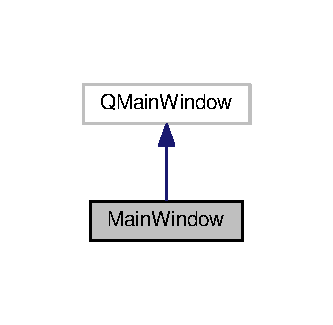
\includegraphics[width=160pt]{class_main_window__inherit__graph}
\end{center}
\end{figure}


Collaboration diagram for Main\+Window\+:
\nopagebreak
\begin{figure}[H]
\begin{center}
\leavevmode
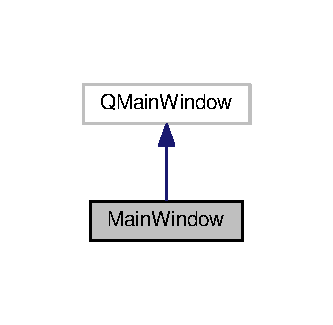
\includegraphics[width=160pt]{class_main_window__coll__graph}
\end{center}
\end{figure}
\subsection*{Public Slots}
\begin{DoxyCompactItemize}
\item 
void \hyperlink{class_main_window_a0edca0c59fb238bea02b248c90b89698}{show\+Message} (Q\+String msg)
\end{DoxyCompactItemize}
\subsection*{Public Member Functions}
\begin{DoxyCompactItemize}
\item 
\hyperlink{class_main_window_a8b244be8b7b7db1b08de2a2acb9409db}{Main\+Window} (Q\+Widget $\ast$parent=0)
\item 
\hyperlink{class_main_window_ae98d00a93bc118200eeef9f9bba1dba7}{$\sim$\+Main\+Window} ()
\end{DoxyCompactItemize}


\subsection{Constructor \& Destructor Documentation}
\index{Main\+Window@{Main\+Window}!Main\+Window@{Main\+Window}}
\index{Main\+Window@{Main\+Window}!Main\+Window@{Main\+Window}}
\subsubsection[{\texorpdfstring{Main\+Window(\+Q\+Widget $\ast$parent=0)}{MainWindow(QWidget *parent=0)}}]{\setlength{\rightskip}{0pt plus 5cm}Main\+Window\+::\+Main\+Window (
\begin{DoxyParamCaption}
\item[{Q\+Widget $\ast$}]{parent = {\ttfamily 0}}
\end{DoxyParamCaption}
)\hspace{0.3cm}{\ttfamily [explicit]}}\hypertarget{class_main_window_a8b244be8b7b7db1b08de2a2acb9409db}{}\label{class_main_window_a8b244be8b7b7db1b08de2a2acb9409db}
\index{Main\+Window@{Main\+Window}!````~Main\+Window@{$\sim$\+Main\+Window}}
\index{````~Main\+Window@{$\sim$\+Main\+Window}!Main\+Window@{Main\+Window}}
\subsubsection[{\texorpdfstring{$\sim$\+Main\+Window()}{~MainWindow()}}]{\setlength{\rightskip}{0pt plus 5cm}Main\+Window\+::$\sim$\+Main\+Window (
\begin{DoxyParamCaption}
{}
\end{DoxyParamCaption}
)}\hypertarget{class_main_window_ae98d00a93bc118200eeef9f9bba1dba7}{}\label{class_main_window_ae98d00a93bc118200eeef9f9bba1dba7}


\subsection{Member Function Documentation}
\index{Main\+Window@{Main\+Window}!show\+Message@{show\+Message}}
\index{show\+Message@{show\+Message}!Main\+Window@{Main\+Window}}
\subsubsection[{\texorpdfstring{show\+Message}{showMessage}}]{\setlength{\rightskip}{0pt plus 5cm}void Main\+Window\+::show\+Message (
\begin{DoxyParamCaption}
\item[{Q\+String}]{msg}
\end{DoxyParamCaption}
)\hspace{0.3cm}{\ttfamily [slot]}}\hypertarget{class_main_window_a0edca0c59fb238bea02b248c90b89698}{}\label{class_main_window_a0edca0c59fb238bea02b248c90b89698}


The documentation for this class was generated from the following files\+:\begin{DoxyCompactItemize}
\item 
Qt\+Tcp\+Server/\hyperlink{mainwindow_8h}{mainwindow.\+h}\item 
Qt\+Tcp\+Server/\hyperlink{mainwindow_8cpp}{mainwindow.\+cpp}\end{DoxyCompactItemize}

\hypertarget{class_ui_1_1_main_window}{}\section{Ui\+:\+:Main\+Window Class Reference}
\label{class_ui_1_1_main_window}\index{Ui\+::\+Main\+Window@{Ui\+::\+Main\+Window}}


{\ttfamily \#include $<$ui\+\_\+mainwindow.\+h$>$}



Inheritance diagram for Ui\+:\+:Main\+Window\+:
\nopagebreak
\begin{figure}[H]
\begin{center}
\leavevmode
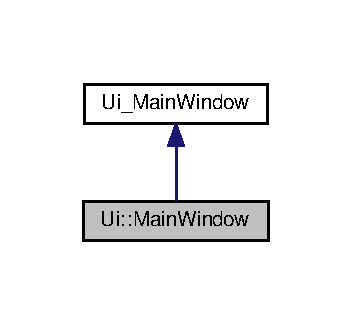
\includegraphics[width=169pt]{class_ui_1_1_main_window__inherit__graph}
\end{center}
\end{figure}


Collaboration diagram for Ui\+:\+:Main\+Window\+:
\nopagebreak
\begin{figure}[H]
\begin{center}
\leavevmode
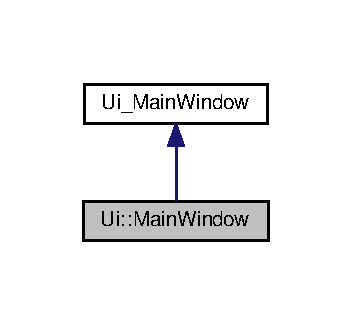
\includegraphics[width=169pt]{class_ui_1_1_main_window__coll__graph}
\end{center}
\end{figure}
\subsection*{Additional Inherited Members}


The documentation for this class was generated from the following file\+:\begin{DoxyCompactItemize}
\item 
Qt\+Tcp\+Server/\hyperlink{ui__mainwindow_8h}{ui\+\_\+mainwindow.\+h}\end{DoxyCompactItemize}

\hypertarget{class_my_server}{}\section{My\+Server Class Reference}
\label{class_my_server}\index{My\+Server@{My\+Server}}


The \hyperlink{class_my_server}{My\+Server} class inicia um servidor T\+CP capaz de \char`\"{}ouvir\char`\"{} a porta 1234.  




{\ttfamily \#include $<$myserver.\+h$>$}



Inheritance diagram for My\+Server\+:
\nopagebreak
\begin{figure}[H]
\begin{center}
\leavevmode
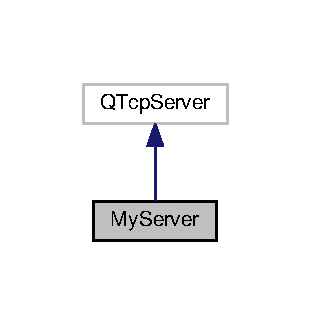
\includegraphics[width=149pt]{class_my_server__inherit__graph}
\end{center}
\end{figure}


Collaboration diagram for My\+Server\+:
\nopagebreak
\begin{figure}[H]
\begin{center}
\leavevmode
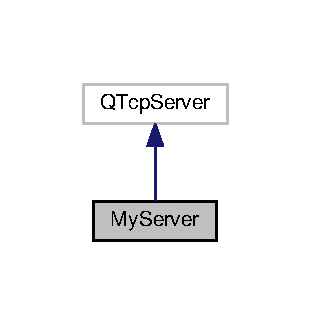
\includegraphics[width=149pt]{class_my_server__coll__graph}
\end{center}
\end{figure}
\subsection*{Public Slots}
\begin{DoxyCompactItemize}
\item 
void \hyperlink{class_my_server_ac795ee6f1607c0fa4e635a0da2bf2164}{receive\+Msg} (Q\+String str)
\end{DoxyCompactItemize}
\subsection*{Signals}
\begin{DoxyCompactItemize}
\item 
void \hyperlink{class_my_server_a2b884bce37840b1b461363a37b463b30}{message} (Q\+String)
\end{DoxyCompactItemize}
\subsection*{Public Member Functions}
\begin{DoxyCompactItemize}
\item 
\hyperlink{class_my_server_ac9e5ca7b551a5df90d5b39260f7e5404}{My\+Server} (Q\+Object $\ast$parent=0)
\begin{DoxyCompactList}\small\item\em \hyperlink{class_my_server}{My\+Server} é o construtor da classe. \end{DoxyCompactList}\item 
void \hyperlink{class_my_server_a962f0e205a0aaf08b12d50d1315a8c90}{start\+Server} ()
\begin{DoxyCompactList}\small\item\em Start\+Server start the T\+CP server. \end{DoxyCompactList}\item 
Q\+String\+List \hyperlink{class_my_server_ac10d498dcc2b5d691f131f17b6602a59}{get\+I\+P\+List} ()
\begin{DoxyCompactList}\small\item\em get\+I\+P\+List return a list of I\+Ps used by server \end{DoxyCompactList}\end{DoxyCompactItemize}
\subsection*{Protected Member Functions}
\begin{DoxyCompactItemize}
\item 
void \hyperlink{class_my_server_a635c7a1e6817285ffb1a2a3842df010b}{incoming\+Connection} (qintptr socket\+Descriptor)
\begin{DoxyCompactList}\small\item\em incoming\+Connection decide o que fazer quando uma nova conexao é iniciada \end{DoxyCompactList}\end{DoxyCompactItemize}


\subsection{Detailed Description}
The \hyperlink{class_my_server}{My\+Server} class inicia um servidor T\+CP capaz de \char`\"{}ouvir\char`\"{} a porta 1234. 

\subsection{Constructor \& Destructor Documentation}
\index{My\+Server@{My\+Server}!My\+Server@{My\+Server}}
\index{My\+Server@{My\+Server}!My\+Server@{My\+Server}}
\subsubsection[{\texorpdfstring{My\+Server(\+Q\+Object $\ast$parent=0)}{MyServer(QObject *parent=0)}}]{\setlength{\rightskip}{0pt plus 5cm}My\+Server\+::\+My\+Server (
\begin{DoxyParamCaption}
\item[{Q\+Object $\ast$}]{parent = {\ttfamily 0}}
\end{DoxyParamCaption}
)}\hypertarget{class_my_server_ac9e5ca7b551a5df90d5b39260f7e5404}{}\label{class_my_server_ac9e5ca7b551a5df90d5b39260f7e5404}


\hyperlink{class_my_server}{My\+Server} é o construtor da classe. 


\begin{DoxyParams}{Parameters}
{\em parent} & eh o pai do objeto (nao usado) \\
\hline
\end{DoxyParams}


\subsection{Member Function Documentation}
\index{My\+Server@{My\+Server}!get\+I\+P\+List@{get\+I\+P\+List}}
\index{get\+I\+P\+List@{get\+I\+P\+List}!My\+Server@{My\+Server}}
\subsubsection[{\texorpdfstring{get\+I\+P\+List()}{getIPList()}}]{\setlength{\rightskip}{0pt plus 5cm}Q\+String\+List My\+Server\+::get\+I\+P\+List (
\begin{DoxyParamCaption}
{}
\end{DoxyParamCaption}
)}\hypertarget{class_my_server_ac10d498dcc2b5d691f131f17b6602a59}{}\label{class_my_server_ac10d498dcc2b5d691f131f17b6602a59}


get\+I\+P\+List return a list of I\+Ps used by server 

\begin{DoxyReturn}{Returns}

\end{DoxyReturn}
\index{My\+Server@{My\+Server}!incoming\+Connection@{incoming\+Connection}}
\index{incoming\+Connection@{incoming\+Connection}!My\+Server@{My\+Server}}
\subsubsection[{\texorpdfstring{incoming\+Connection(qintptr socket\+Descriptor)}{incomingConnection(qintptr socketDescriptor)}}]{\setlength{\rightskip}{0pt plus 5cm}void My\+Server\+::incoming\+Connection (
\begin{DoxyParamCaption}
\item[{qintptr}]{socket\+Descriptor}
\end{DoxyParamCaption}
)\hspace{0.3cm}{\ttfamily [protected]}}\hypertarget{class_my_server_a635c7a1e6817285ffb1a2a3842df010b}{}\label{class_my_server_a635c7a1e6817285ffb1a2a3842df010b}


incoming\+Connection decide o que fazer quando uma nova conexao é iniciada 


\begin{DoxyParams}{Parameters}
{\em socket\+Descriptor} & é o identificador do socket para a conexao \\
\hline
\end{DoxyParams}
\index{My\+Server@{My\+Server}!message@{message}}
\index{message@{message}!My\+Server@{My\+Server}}
\subsubsection[{\texorpdfstring{message}{message}}]{\setlength{\rightskip}{0pt plus 5cm}void My\+Server\+::message (
\begin{DoxyParamCaption}
\item[{Q\+String}]{\+\_\+t1}
\end{DoxyParamCaption}
)\hspace{0.3cm}{\ttfamily [signal]}}\hypertarget{class_my_server_a2b884bce37840b1b461363a37b463b30}{}\label{class_my_server_a2b884bce37840b1b461363a37b463b30}
\index{My\+Server@{My\+Server}!receive\+Msg@{receive\+Msg}}
\index{receive\+Msg@{receive\+Msg}!My\+Server@{My\+Server}}
\subsubsection[{\texorpdfstring{receive\+Msg}{receiveMsg}}]{\setlength{\rightskip}{0pt plus 5cm}void My\+Server\+::receive\+Msg (
\begin{DoxyParamCaption}
\item[{Q\+String}]{str}
\end{DoxyParamCaption}
)\hspace{0.3cm}{\ttfamily [slot]}}\hypertarget{class_my_server_ac795ee6f1607c0fa4e635a0da2bf2164}{}\label{class_my_server_ac795ee6f1607c0fa4e635a0da2bf2164}
\index{My\+Server@{My\+Server}!start\+Server@{start\+Server}}
\index{start\+Server@{start\+Server}!My\+Server@{My\+Server}}
\subsubsection[{\texorpdfstring{start\+Server()}{startServer()}}]{\setlength{\rightskip}{0pt plus 5cm}void My\+Server\+::start\+Server (
\begin{DoxyParamCaption}
{}
\end{DoxyParamCaption}
)}\hypertarget{class_my_server_a962f0e205a0aaf08b12d50d1315a8c90}{}\label{class_my_server_a962f0e205a0aaf08b12d50d1315a8c90}


Start\+Server start the T\+CP server. 



The documentation for this class was generated from the following files\+:\begin{DoxyCompactItemize}
\item 
Qt\+Tcp\+Server/\hyperlink{myserver_8h}{myserver.\+h}\item 
Qt\+Tcp\+Server/\hyperlink{moc__myserver_8cpp}{moc\+\_\+myserver.\+cpp}\item 
Qt\+Tcp\+Server/\hyperlink{myserver_8cpp}{myserver.\+cpp}\end{DoxyCompactItemize}

\hypertarget{class_my_thread}{}\section{My\+Thread Class Reference}
\label{class_my_thread}\index{My\+Thread@{My\+Thread}}


The \hyperlink{class_my_thread}{My\+Thread} class cria uma thread que lida com o tratamento de uma conexao T\+CP de entrada.  




{\ttfamily \#include $<$mythread.\+h$>$}



Inheritance diagram for My\+Thread\+:
\nopagebreak
\begin{figure}[H]
\begin{center}
\leavevmode
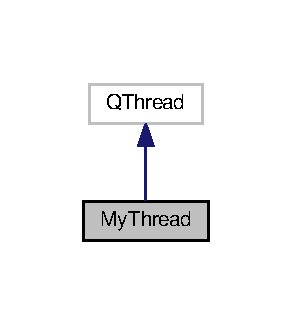
\includegraphics[width=140pt]{class_my_thread__inherit__graph}
\end{center}
\end{figure}


Collaboration diagram for My\+Thread\+:
\nopagebreak
\begin{figure}[H]
\begin{center}
\leavevmode
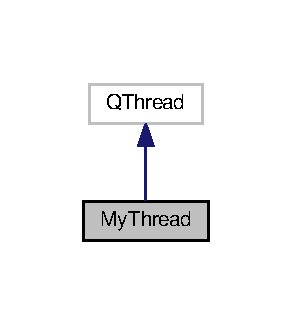
\includegraphics[width=140pt]{class_my_thread__coll__graph}
\end{center}
\end{figure}
\subsection*{Public Slots}
\begin{DoxyCompactItemize}
\item 
void \hyperlink{class_my_thread_a277618fdd448b927f2e250c2076fc176}{ready\+Read} ()
\item 
void \hyperlink{class_my_thread_a447710039787ae20134a9b572487840f}{disconnected} ()
\end{DoxyCompactItemize}
\subsection*{Signals}
\begin{DoxyCompactItemize}
\item 
void \hyperlink{class_my_thread_aebf11d93838f22c9547d0c6aa97002be}{error} (Q\+Tcp\+Socket\+::\+Socket\+Error socketerror)
\item 
void \hyperlink{class_my_thread_ae49528d4ec1b2208240f707f5aa74adf}{message} (Q\+String)
\end{DoxyCompactItemize}
\subsection*{Public Member Functions}
\begin{DoxyCompactItemize}
\item 
\hyperlink{class_my_thread_ac1b04b0fa6b32038e810c7105ef762f6}{My\+Thread} (int ID, Q\+Object $\ast$parent, \hyperlink{class_data_storage}{Data\+Storage} $\ast$storage)
\begin{DoxyCompactList}\small\item\em \hyperlink{class_my_thread}{My\+Thread} eh o construtor da classe. \end{DoxyCompactList}\item 
void \hyperlink{class_my_thread_a48f2e366e852087c53705f64e1ee65c2}{run} ()
\end{DoxyCompactItemize}


\subsection{Detailed Description}
The \hyperlink{class_my_thread}{My\+Thread} class cria uma thread que lida com o tratamento de uma conexao T\+CP de entrada. 

\subsection{Constructor \& Destructor Documentation}
\index{My\+Thread@{My\+Thread}!My\+Thread@{My\+Thread}}
\index{My\+Thread@{My\+Thread}!My\+Thread@{My\+Thread}}
\subsubsection[{\texorpdfstring{My\+Thread(int I\+D, Q\+Object $\ast$parent, Data\+Storage $\ast$storage)}{MyThread(int ID, QObject *parent, DataStorage *storage)}}]{\setlength{\rightskip}{0pt plus 5cm}My\+Thread\+::\+My\+Thread (
\begin{DoxyParamCaption}
\item[{int}]{ID, }
\item[{Q\+Object $\ast$}]{parent, }
\item[{{\bf Data\+Storage} $\ast$}]{storage}
\end{DoxyParamCaption}
)}\hypertarget{class_my_thread_ac1b04b0fa6b32038e810c7105ef762f6}{}\label{class_my_thread_ac1b04b0fa6b32038e810c7105ef762f6}


\hyperlink{class_my_thread}{My\+Thread} eh o construtor da classe. 


\begin{DoxyParams}{Parameters}
{\em ID} & eh o identificador da thread \\
\hline
{\em parent} & \\
\hline
{\em storage} & \\
\hline
\end{DoxyParams}


\subsection{Member Function Documentation}
\index{My\+Thread@{My\+Thread}!disconnected@{disconnected}}
\index{disconnected@{disconnected}!My\+Thread@{My\+Thread}}
\subsubsection[{\texorpdfstring{disconnected}{disconnected}}]{\setlength{\rightskip}{0pt plus 5cm}void My\+Thread\+::disconnected (
\begin{DoxyParamCaption}
{}
\end{DoxyParamCaption}
)\hspace{0.3cm}{\ttfamily [slot]}}\hypertarget{class_my_thread_a447710039787ae20134a9b572487840f}{}\label{class_my_thread_a447710039787ae20134a9b572487840f}
\index{My\+Thread@{My\+Thread}!error@{error}}
\index{error@{error}!My\+Thread@{My\+Thread}}
\subsubsection[{\texorpdfstring{error}{error}}]{\setlength{\rightskip}{0pt plus 5cm}void My\+Thread\+::error (
\begin{DoxyParamCaption}
\item[{Q\+Tcp\+Socket\+::\+Socket\+Error}]{socketerror}
\end{DoxyParamCaption}
)\hspace{0.3cm}{\ttfamily [signal]}}\hypertarget{class_my_thread_aebf11d93838f22c9547d0c6aa97002be}{}\label{class_my_thread_aebf11d93838f22c9547d0c6aa97002be}
\index{My\+Thread@{My\+Thread}!message@{message}}
\index{message@{message}!My\+Thread@{My\+Thread}}
\subsubsection[{\texorpdfstring{message}{message}}]{\setlength{\rightskip}{0pt plus 5cm}void My\+Thread\+::message (
\begin{DoxyParamCaption}
\item[{Q\+String}]{\+\_\+t1}
\end{DoxyParamCaption}
)\hspace{0.3cm}{\ttfamily [signal]}}\hypertarget{class_my_thread_ae49528d4ec1b2208240f707f5aa74adf}{}\label{class_my_thread_ae49528d4ec1b2208240f707f5aa74adf}
\index{My\+Thread@{My\+Thread}!ready\+Read@{ready\+Read}}
\index{ready\+Read@{ready\+Read}!My\+Thread@{My\+Thread}}
\subsubsection[{\texorpdfstring{ready\+Read}{readyRead}}]{\setlength{\rightskip}{0pt plus 5cm}void My\+Thread\+::ready\+Read (
\begin{DoxyParamCaption}
{}
\end{DoxyParamCaption}
)\hspace{0.3cm}{\ttfamily [slot]}}\hypertarget{class_my_thread_a277618fdd448b927f2e250c2076fc176}{}\label{class_my_thread_a277618fdd448b927f2e250c2076fc176}
\index{My\+Thread@{My\+Thread}!run@{run}}
\index{run@{run}!My\+Thread@{My\+Thread}}
\subsubsection[{\texorpdfstring{run()}{run()}}]{\setlength{\rightskip}{0pt plus 5cm}void My\+Thread\+::run (
\begin{DoxyParamCaption}
{}
\end{DoxyParamCaption}
)}\hypertarget{class_my_thread_a48f2e366e852087c53705f64e1ee65c2}{}\label{class_my_thread_a48f2e366e852087c53705f64e1ee65c2}


The documentation for this class was generated from the following files\+:\begin{DoxyCompactItemize}
\item 
Qt\+Tcp\+Server/\hyperlink{mythread_8h}{mythread.\+h}\item 
Qt\+Tcp\+Server/\hyperlink{moc__mythread_8cpp}{moc\+\_\+mythread.\+cpp}\item 
Qt\+Tcp\+Server/\hyperlink{mythread_8cpp}{mythread.\+cpp}\end{DoxyCompactItemize}

\hypertarget{structqt__meta__stringdata___main_window__t}{}\section{qt\+\_\+meta\+\_\+stringdata\+\_\+\+Main\+Window\+\_\+t Struct Reference}
\label{structqt__meta__stringdata___main_window__t}\index{qt\+\_\+meta\+\_\+stringdata\+\_\+\+Main\+Window\+\_\+t@{qt\+\_\+meta\+\_\+stringdata\+\_\+\+Main\+Window\+\_\+t}}
\subsection*{Public Attributes}
\begin{DoxyCompactItemize}
\item 
Q\+Byte\+Array\+Data \hyperlink{structqt__meta__stringdata___main_window__t_a332d7fa058028f7613b5ba68abb5a7fe}{data} \mbox{[}4\mbox{]}
\item 
char \hyperlink{structqt__meta__stringdata___main_window__t_a10e266ffded4c5e956d35d922fa94828}{stringdata0} \mbox{[}28\mbox{]}
\end{DoxyCompactItemize}


\subsection{Member Data Documentation}
\index{qt\+\_\+meta\+\_\+stringdata\+\_\+\+Main\+Window\+\_\+t@{qt\+\_\+meta\+\_\+stringdata\+\_\+\+Main\+Window\+\_\+t}!data@{data}}
\index{data@{data}!qt\+\_\+meta\+\_\+stringdata\+\_\+\+Main\+Window\+\_\+t@{qt\+\_\+meta\+\_\+stringdata\+\_\+\+Main\+Window\+\_\+t}}
\subsubsection[{\texorpdfstring{data}{data}}]{\setlength{\rightskip}{0pt plus 5cm}Q\+Byte\+Array\+Data qt\+\_\+meta\+\_\+stringdata\+\_\+\+Main\+Window\+\_\+t\+::data\mbox{[}4\mbox{]}}\hypertarget{structqt__meta__stringdata___main_window__t_a332d7fa058028f7613b5ba68abb5a7fe}{}\label{structqt__meta__stringdata___main_window__t_a332d7fa058028f7613b5ba68abb5a7fe}
\index{qt\+\_\+meta\+\_\+stringdata\+\_\+\+Main\+Window\+\_\+t@{qt\+\_\+meta\+\_\+stringdata\+\_\+\+Main\+Window\+\_\+t}!stringdata0@{stringdata0}}
\index{stringdata0@{stringdata0}!qt\+\_\+meta\+\_\+stringdata\+\_\+\+Main\+Window\+\_\+t@{qt\+\_\+meta\+\_\+stringdata\+\_\+\+Main\+Window\+\_\+t}}
\subsubsection[{\texorpdfstring{stringdata0}{stringdata0}}]{\setlength{\rightskip}{0pt plus 5cm}char qt\+\_\+meta\+\_\+stringdata\+\_\+\+Main\+Window\+\_\+t\+::stringdata0\mbox{[}28\mbox{]}}\hypertarget{structqt__meta__stringdata___main_window__t_a10e266ffded4c5e956d35d922fa94828}{}\label{structqt__meta__stringdata___main_window__t_a10e266ffded4c5e956d35d922fa94828}


The documentation for this struct was generated from the following file\+:\begin{DoxyCompactItemize}
\item 
Qt\+Tcp\+Server/\hyperlink{moc__mainwindow_8cpp}{moc\+\_\+mainwindow.\+cpp}\end{DoxyCompactItemize}

\hypertarget{structqt__meta__stringdata___my_server__t}{}\section{qt\+\_\+meta\+\_\+stringdata\+\_\+\+My\+Server\+\_\+t Struct Reference}
\label{structqt__meta__stringdata___my_server__t}\index{qt\+\_\+meta\+\_\+stringdata\+\_\+\+My\+Server\+\_\+t@{qt\+\_\+meta\+\_\+stringdata\+\_\+\+My\+Server\+\_\+t}}
\subsection*{Public Attributes}
\begin{DoxyCompactItemize}
\item 
Q\+Byte\+Array\+Data \hyperlink{structqt__meta__stringdata___my_server__t_ab15722048201cc80be7f2b05eece64e9}{data} \mbox{[}5\mbox{]}
\item 
char \hyperlink{structqt__meta__stringdata___my_server__t_a54652770c5771b1f6db92acb7932b3dd}{stringdata0} \mbox{[}33\mbox{]}
\end{DoxyCompactItemize}


\subsection{Member Data Documentation}
\index{qt\+\_\+meta\+\_\+stringdata\+\_\+\+My\+Server\+\_\+t@{qt\+\_\+meta\+\_\+stringdata\+\_\+\+My\+Server\+\_\+t}!data@{data}}
\index{data@{data}!qt\+\_\+meta\+\_\+stringdata\+\_\+\+My\+Server\+\_\+t@{qt\+\_\+meta\+\_\+stringdata\+\_\+\+My\+Server\+\_\+t}}
\subsubsection[{\texorpdfstring{data}{data}}]{\setlength{\rightskip}{0pt plus 5cm}Q\+Byte\+Array\+Data qt\+\_\+meta\+\_\+stringdata\+\_\+\+My\+Server\+\_\+t\+::data\mbox{[}5\mbox{]}}\hypertarget{structqt__meta__stringdata___my_server__t_ab15722048201cc80be7f2b05eece64e9}{}\label{structqt__meta__stringdata___my_server__t_ab15722048201cc80be7f2b05eece64e9}
\index{qt\+\_\+meta\+\_\+stringdata\+\_\+\+My\+Server\+\_\+t@{qt\+\_\+meta\+\_\+stringdata\+\_\+\+My\+Server\+\_\+t}!stringdata0@{stringdata0}}
\index{stringdata0@{stringdata0}!qt\+\_\+meta\+\_\+stringdata\+\_\+\+My\+Server\+\_\+t@{qt\+\_\+meta\+\_\+stringdata\+\_\+\+My\+Server\+\_\+t}}
\subsubsection[{\texorpdfstring{stringdata0}{stringdata0}}]{\setlength{\rightskip}{0pt plus 5cm}char qt\+\_\+meta\+\_\+stringdata\+\_\+\+My\+Server\+\_\+t\+::stringdata0\mbox{[}33\mbox{]}}\hypertarget{structqt__meta__stringdata___my_server__t_a54652770c5771b1f6db92acb7932b3dd}{}\label{structqt__meta__stringdata___my_server__t_a54652770c5771b1f6db92acb7932b3dd}


The documentation for this struct was generated from the following file\+:\begin{DoxyCompactItemize}
\item 
Qt\+Tcp\+Server/\hyperlink{moc__myserver_8cpp}{moc\+\_\+myserver.\+cpp}\end{DoxyCompactItemize}

\hypertarget{structqt__meta__stringdata___my_thread__t}{}\section{qt\+\_\+meta\+\_\+stringdata\+\_\+\+My\+Thread\+\_\+t Struct Reference}
\label{structqt__meta__stringdata___my_thread__t}\index{qt\+\_\+meta\+\_\+stringdata\+\_\+\+My\+Thread\+\_\+t@{qt\+\_\+meta\+\_\+stringdata\+\_\+\+My\+Thread\+\_\+t}}
\subsection*{Public Attributes}
\begin{DoxyCompactItemize}
\item 
Q\+Byte\+Array\+Data \hyperlink{structqt__meta__stringdata___my_thread__t_ab5607f1078333a9d42458336e4f735dd}{data} \mbox{[}8\mbox{]}
\item 
char \hyperlink{structqt__meta__stringdata___my_thread__t_aa80f739ca8c1b5cfcf28f7f8d8666688}{stringdata0} \mbox{[}83\mbox{]}
\end{DoxyCompactItemize}


\subsection{Member Data Documentation}
\index{qt\+\_\+meta\+\_\+stringdata\+\_\+\+My\+Thread\+\_\+t@{qt\+\_\+meta\+\_\+stringdata\+\_\+\+My\+Thread\+\_\+t}!data@{data}}
\index{data@{data}!qt\+\_\+meta\+\_\+stringdata\+\_\+\+My\+Thread\+\_\+t@{qt\+\_\+meta\+\_\+stringdata\+\_\+\+My\+Thread\+\_\+t}}
\subsubsection[{\texorpdfstring{data}{data}}]{\setlength{\rightskip}{0pt plus 5cm}Q\+Byte\+Array\+Data qt\+\_\+meta\+\_\+stringdata\+\_\+\+My\+Thread\+\_\+t\+::data\mbox{[}8\mbox{]}}\hypertarget{structqt__meta__stringdata___my_thread__t_ab5607f1078333a9d42458336e4f735dd}{}\label{structqt__meta__stringdata___my_thread__t_ab5607f1078333a9d42458336e4f735dd}
\index{qt\+\_\+meta\+\_\+stringdata\+\_\+\+My\+Thread\+\_\+t@{qt\+\_\+meta\+\_\+stringdata\+\_\+\+My\+Thread\+\_\+t}!stringdata0@{stringdata0}}
\index{stringdata0@{stringdata0}!qt\+\_\+meta\+\_\+stringdata\+\_\+\+My\+Thread\+\_\+t@{qt\+\_\+meta\+\_\+stringdata\+\_\+\+My\+Thread\+\_\+t}}
\subsubsection[{\texorpdfstring{stringdata0}{stringdata0}}]{\setlength{\rightskip}{0pt plus 5cm}char qt\+\_\+meta\+\_\+stringdata\+\_\+\+My\+Thread\+\_\+t\+::stringdata0\mbox{[}83\mbox{]}}\hypertarget{structqt__meta__stringdata___my_thread__t_aa80f739ca8c1b5cfcf28f7f8d8666688}{}\label{structqt__meta__stringdata___my_thread__t_aa80f739ca8c1b5cfcf28f7f8d8666688}


The documentation for this struct was generated from the following file\+:\begin{DoxyCompactItemize}
\item 
Qt\+Tcp\+Server/\hyperlink{moc__mythread_8cpp}{moc\+\_\+mythread.\+cpp}\end{DoxyCompactItemize}

\hypertarget{struct_range_test}{}\section{Range\+Test Struct Reference}
\label{struct_range_test}\index{Range\+Test@{Range\+Test}}
\subsection*{Public Member Functions}
\begin{DoxyCompactItemize}
\item 
\hyperlink{struct_range_test_a9d96f82c111ffd4d2747416b90306791}{Range\+Test} (qint64 \+\_\+limit)
\item 
bool \hyperlink{struct_range_test_add496768a566e04219e840ee25e829d7}{operator()} (qint64 n)
\end{DoxyCompactItemize}
\subsection*{Public Attributes}
\begin{DoxyCompactItemize}
\item 
qint64 \hyperlink{struct_range_test_a638ebd61c0447db219f10cd1473ab364}{limit}
\end{DoxyCompactItemize}


\subsection{Constructor \& Destructor Documentation}
\index{Range\+Test@{Range\+Test}!Range\+Test@{Range\+Test}}
\index{Range\+Test@{Range\+Test}!Range\+Test@{Range\+Test}}
\subsubsection[{\texorpdfstring{Range\+Test(qint64 \+\_\+limit)}{RangeTest(qint64 _limit)}}]{\setlength{\rightskip}{0pt plus 5cm}Range\+Test\+::\+Range\+Test (
\begin{DoxyParamCaption}
\item[{qint64}]{\+\_\+limit}
\end{DoxyParamCaption}
)\hspace{0.3cm}{\ttfamily [inline]}}\hypertarget{struct_range_test_a9d96f82c111ffd4d2747416b90306791}{}\label{struct_range_test_a9d96f82c111ffd4d2747416b90306791}


\subsection{Member Function Documentation}
\index{Range\+Test@{Range\+Test}!operator()@{operator()}}
\index{operator()@{operator()}!Range\+Test@{Range\+Test}}
\subsubsection[{\texorpdfstring{operator()(qint64 n)}{operator()(qint64 n)}}]{\setlength{\rightskip}{0pt plus 5cm}bool Range\+Test\+::operator() (
\begin{DoxyParamCaption}
\item[{qint64}]{n}
\end{DoxyParamCaption}
)\hspace{0.3cm}{\ttfamily [inline]}}\hypertarget{struct_range_test_add496768a566e04219e840ee25e829d7}{}\label{struct_range_test_add496768a566e04219e840ee25e829d7}


\subsection{Member Data Documentation}
\index{Range\+Test@{Range\+Test}!limit@{limit}}
\index{limit@{limit}!Range\+Test@{Range\+Test}}
\subsubsection[{\texorpdfstring{limit}{limit}}]{\setlength{\rightskip}{0pt plus 5cm}qint64 Range\+Test\+::limit}\hypertarget{struct_range_test_a638ebd61c0447db219f10cd1473ab364}{}\label{struct_range_test_a638ebd61c0447db219f10cd1473ab364}


The documentation for this struct was generated from the following file\+:\begin{DoxyCompactItemize}
\item 
Qt\+Tcp\+Server/\hyperlink{datastorage_8cpp}{datastorage.\+cpp}\end{DoxyCompactItemize}

\hypertarget{class_ui___main_window}{}\section{Ui\+\_\+\+Main\+Window Class Reference}
\label{class_ui___main_window}\index{Ui\+\_\+\+Main\+Window@{Ui\+\_\+\+Main\+Window}}


{\ttfamily \#include $<$ui\+\_\+mainwindow.\+h$>$}



Inheritance diagram for Ui\+\_\+\+Main\+Window\+:
\nopagebreak
\begin{figure}[H]
\begin{center}
\leavevmode
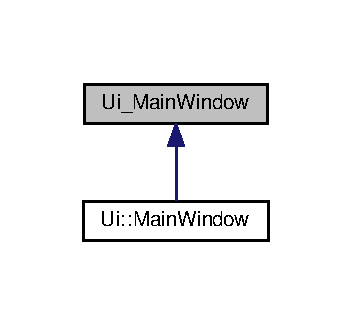
\includegraphics[width=169pt]{class_ui___main_window__inherit__graph}
\end{center}
\end{figure}
\subsection*{Public Member Functions}
\begin{DoxyCompactItemize}
\item 
void \hyperlink{class_ui___main_window_acf4a0872c4c77d8f43a2ec66ed849b58}{setup\+Ui} (Q\+Main\+Window $\ast$\hyperlink{class_main_window}{Main\+Window})
\item 
void \hyperlink{class_ui___main_window_a097dd160c3534a204904cb374412c618}{retranslate\+Ui} (Q\+Main\+Window $\ast$\hyperlink{class_main_window}{Main\+Window})
\end{DoxyCompactItemize}
\subsection*{Public Attributes}
\begin{DoxyCompactItemize}
\item 
Q\+Widget $\ast$ \hyperlink{class_ui___main_window_a30075506c2116c3ed4ff25e07ae75f81}{central\+Widget}
\item 
Q\+H\+Box\+Layout $\ast$ \hyperlink{class_ui___main_window_a03ce63974cc69b067c91bbf285cceca8}{horizontal\+Layout\+\_\+3}
\item 
Q\+Group\+Box $\ast$ \hyperlink{class_ui___main_window_aef7cb3be8cecfc9aaf98f036a98781ce}{group\+Box}
\item 
Q\+H\+Box\+Layout $\ast$ \hyperlink{class_ui___main_window_acd6fdc9ebacc4b25b834162380d75ce8}{horizontal\+Layout}
\item 
Q\+List\+Widget $\ast$ \hyperlink{class_ui___main_window_ae647a15635ba8a0e5d5aec475db99d8f}{list\+Widget}
\item 
Q\+Group\+Box $\ast$ \hyperlink{class_ui___main_window_abb28acde35ffce4d0e6152579df2cbc3}{group\+Box\+\_\+2}
\item 
Q\+H\+Box\+Layout $\ast$ \hyperlink{class_ui___main_window_a80867018070156432923d0266cc9fe25}{horizontal\+Layout\+\_\+2}
\item 
Q\+Text\+Browser $\ast$ \hyperlink{class_ui___main_window_a2c789c07fa5fc1cee05aae8df52bb02d}{text\+Browser}
\item 
Q\+Menu\+Bar $\ast$ \hyperlink{class_ui___main_window_a2be1c24ec9adfca18e1dcc951931457f}{menu\+Bar}
\item 
Q\+Tool\+Bar $\ast$ \hyperlink{class_ui___main_window_a5172877001c8c7b4e0f6de50421867d1}{main\+Tool\+Bar}
\item 
Q\+Status\+Bar $\ast$ \hyperlink{class_ui___main_window_a50fa481337604bcc8bf68de18ab16ecd}{status\+Bar}
\end{DoxyCompactItemize}


\subsection{Member Function Documentation}
\index{Ui\+\_\+\+Main\+Window@{Ui\+\_\+\+Main\+Window}!retranslate\+Ui@{retranslate\+Ui}}
\index{retranslate\+Ui@{retranslate\+Ui}!Ui\+\_\+\+Main\+Window@{Ui\+\_\+\+Main\+Window}}
\subsubsection[{\texorpdfstring{retranslate\+Ui(\+Q\+Main\+Window $\ast$\+Main\+Window)}{retranslateUi(QMainWindow *MainWindow)}}]{\setlength{\rightskip}{0pt plus 5cm}void Ui\+\_\+\+Main\+Window\+::retranslate\+Ui (
\begin{DoxyParamCaption}
\item[{Q\+Main\+Window $\ast$}]{Main\+Window}
\end{DoxyParamCaption}
)\hspace{0.3cm}{\ttfamily [inline]}}\hypertarget{class_ui___main_window_a097dd160c3534a204904cb374412c618}{}\label{class_ui___main_window_a097dd160c3534a204904cb374412c618}
\index{Ui\+\_\+\+Main\+Window@{Ui\+\_\+\+Main\+Window}!setup\+Ui@{setup\+Ui}}
\index{setup\+Ui@{setup\+Ui}!Ui\+\_\+\+Main\+Window@{Ui\+\_\+\+Main\+Window}}
\subsubsection[{\texorpdfstring{setup\+Ui(\+Q\+Main\+Window $\ast$\+Main\+Window)}{setupUi(QMainWindow *MainWindow)}}]{\setlength{\rightskip}{0pt plus 5cm}void Ui\+\_\+\+Main\+Window\+::setup\+Ui (
\begin{DoxyParamCaption}
\item[{Q\+Main\+Window $\ast$}]{Main\+Window}
\end{DoxyParamCaption}
)\hspace{0.3cm}{\ttfamily [inline]}}\hypertarget{class_ui___main_window_acf4a0872c4c77d8f43a2ec66ed849b58}{}\label{class_ui___main_window_acf4a0872c4c77d8f43a2ec66ed849b58}


\subsection{Member Data Documentation}
\index{Ui\+\_\+\+Main\+Window@{Ui\+\_\+\+Main\+Window}!central\+Widget@{central\+Widget}}
\index{central\+Widget@{central\+Widget}!Ui\+\_\+\+Main\+Window@{Ui\+\_\+\+Main\+Window}}
\subsubsection[{\texorpdfstring{central\+Widget}{centralWidget}}]{\setlength{\rightskip}{0pt plus 5cm}Q\+Widget$\ast$ Ui\+\_\+\+Main\+Window\+::central\+Widget}\hypertarget{class_ui___main_window_a30075506c2116c3ed4ff25e07ae75f81}{}\label{class_ui___main_window_a30075506c2116c3ed4ff25e07ae75f81}
\index{Ui\+\_\+\+Main\+Window@{Ui\+\_\+\+Main\+Window}!group\+Box@{group\+Box}}
\index{group\+Box@{group\+Box}!Ui\+\_\+\+Main\+Window@{Ui\+\_\+\+Main\+Window}}
\subsubsection[{\texorpdfstring{group\+Box}{groupBox}}]{\setlength{\rightskip}{0pt plus 5cm}Q\+Group\+Box$\ast$ Ui\+\_\+\+Main\+Window\+::group\+Box}\hypertarget{class_ui___main_window_aef7cb3be8cecfc9aaf98f036a98781ce}{}\label{class_ui___main_window_aef7cb3be8cecfc9aaf98f036a98781ce}
\index{Ui\+\_\+\+Main\+Window@{Ui\+\_\+\+Main\+Window}!group\+Box\+\_\+2@{group\+Box\+\_\+2}}
\index{group\+Box\+\_\+2@{group\+Box\+\_\+2}!Ui\+\_\+\+Main\+Window@{Ui\+\_\+\+Main\+Window}}
\subsubsection[{\texorpdfstring{group\+Box\+\_\+2}{groupBox_2}}]{\setlength{\rightskip}{0pt plus 5cm}Q\+Group\+Box$\ast$ Ui\+\_\+\+Main\+Window\+::group\+Box\+\_\+2}\hypertarget{class_ui___main_window_abb28acde35ffce4d0e6152579df2cbc3}{}\label{class_ui___main_window_abb28acde35ffce4d0e6152579df2cbc3}
\index{Ui\+\_\+\+Main\+Window@{Ui\+\_\+\+Main\+Window}!horizontal\+Layout@{horizontal\+Layout}}
\index{horizontal\+Layout@{horizontal\+Layout}!Ui\+\_\+\+Main\+Window@{Ui\+\_\+\+Main\+Window}}
\subsubsection[{\texorpdfstring{horizontal\+Layout}{horizontalLayout}}]{\setlength{\rightskip}{0pt plus 5cm}Q\+H\+Box\+Layout$\ast$ Ui\+\_\+\+Main\+Window\+::horizontal\+Layout}\hypertarget{class_ui___main_window_acd6fdc9ebacc4b25b834162380d75ce8}{}\label{class_ui___main_window_acd6fdc9ebacc4b25b834162380d75ce8}
\index{Ui\+\_\+\+Main\+Window@{Ui\+\_\+\+Main\+Window}!horizontal\+Layout\+\_\+2@{horizontal\+Layout\+\_\+2}}
\index{horizontal\+Layout\+\_\+2@{horizontal\+Layout\+\_\+2}!Ui\+\_\+\+Main\+Window@{Ui\+\_\+\+Main\+Window}}
\subsubsection[{\texorpdfstring{horizontal\+Layout\+\_\+2}{horizontalLayout_2}}]{\setlength{\rightskip}{0pt plus 5cm}Q\+H\+Box\+Layout$\ast$ Ui\+\_\+\+Main\+Window\+::horizontal\+Layout\+\_\+2}\hypertarget{class_ui___main_window_a80867018070156432923d0266cc9fe25}{}\label{class_ui___main_window_a80867018070156432923d0266cc9fe25}
\index{Ui\+\_\+\+Main\+Window@{Ui\+\_\+\+Main\+Window}!horizontal\+Layout\+\_\+3@{horizontal\+Layout\+\_\+3}}
\index{horizontal\+Layout\+\_\+3@{horizontal\+Layout\+\_\+3}!Ui\+\_\+\+Main\+Window@{Ui\+\_\+\+Main\+Window}}
\subsubsection[{\texorpdfstring{horizontal\+Layout\+\_\+3}{horizontalLayout_3}}]{\setlength{\rightskip}{0pt plus 5cm}Q\+H\+Box\+Layout$\ast$ Ui\+\_\+\+Main\+Window\+::horizontal\+Layout\+\_\+3}\hypertarget{class_ui___main_window_a03ce63974cc69b067c91bbf285cceca8}{}\label{class_ui___main_window_a03ce63974cc69b067c91bbf285cceca8}
\index{Ui\+\_\+\+Main\+Window@{Ui\+\_\+\+Main\+Window}!list\+Widget@{list\+Widget}}
\index{list\+Widget@{list\+Widget}!Ui\+\_\+\+Main\+Window@{Ui\+\_\+\+Main\+Window}}
\subsubsection[{\texorpdfstring{list\+Widget}{listWidget}}]{\setlength{\rightskip}{0pt plus 5cm}Q\+List\+Widget$\ast$ Ui\+\_\+\+Main\+Window\+::list\+Widget}\hypertarget{class_ui___main_window_ae647a15635ba8a0e5d5aec475db99d8f}{}\label{class_ui___main_window_ae647a15635ba8a0e5d5aec475db99d8f}
\index{Ui\+\_\+\+Main\+Window@{Ui\+\_\+\+Main\+Window}!main\+Tool\+Bar@{main\+Tool\+Bar}}
\index{main\+Tool\+Bar@{main\+Tool\+Bar}!Ui\+\_\+\+Main\+Window@{Ui\+\_\+\+Main\+Window}}
\subsubsection[{\texorpdfstring{main\+Tool\+Bar}{mainToolBar}}]{\setlength{\rightskip}{0pt plus 5cm}Q\+Tool\+Bar$\ast$ Ui\+\_\+\+Main\+Window\+::main\+Tool\+Bar}\hypertarget{class_ui___main_window_a5172877001c8c7b4e0f6de50421867d1}{}\label{class_ui___main_window_a5172877001c8c7b4e0f6de50421867d1}
\index{Ui\+\_\+\+Main\+Window@{Ui\+\_\+\+Main\+Window}!menu\+Bar@{menu\+Bar}}
\index{menu\+Bar@{menu\+Bar}!Ui\+\_\+\+Main\+Window@{Ui\+\_\+\+Main\+Window}}
\subsubsection[{\texorpdfstring{menu\+Bar}{menuBar}}]{\setlength{\rightskip}{0pt plus 5cm}Q\+Menu\+Bar$\ast$ Ui\+\_\+\+Main\+Window\+::menu\+Bar}\hypertarget{class_ui___main_window_a2be1c24ec9adfca18e1dcc951931457f}{}\label{class_ui___main_window_a2be1c24ec9adfca18e1dcc951931457f}
\index{Ui\+\_\+\+Main\+Window@{Ui\+\_\+\+Main\+Window}!status\+Bar@{status\+Bar}}
\index{status\+Bar@{status\+Bar}!Ui\+\_\+\+Main\+Window@{Ui\+\_\+\+Main\+Window}}
\subsubsection[{\texorpdfstring{status\+Bar}{statusBar}}]{\setlength{\rightskip}{0pt plus 5cm}Q\+Status\+Bar$\ast$ Ui\+\_\+\+Main\+Window\+::status\+Bar}\hypertarget{class_ui___main_window_a50fa481337604bcc8bf68de18ab16ecd}{}\label{class_ui___main_window_a50fa481337604bcc8bf68de18ab16ecd}
\index{Ui\+\_\+\+Main\+Window@{Ui\+\_\+\+Main\+Window}!text\+Browser@{text\+Browser}}
\index{text\+Browser@{text\+Browser}!Ui\+\_\+\+Main\+Window@{Ui\+\_\+\+Main\+Window}}
\subsubsection[{\texorpdfstring{text\+Browser}{textBrowser}}]{\setlength{\rightskip}{0pt plus 5cm}Q\+Text\+Browser$\ast$ Ui\+\_\+\+Main\+Window\+::text\+Browser}\hypertarget{class_ui___main_window_a2c789c07fa5fc1cee05aae8df52bb02d}{}\label{class_ui___main_window_a2c789c07fa5fc1cee05aae8df52bb02d}


The documentation for this class was generated from the following file\+:\begin{DoxyCompactItemize}
\item 
Qt\+Tcp\+Server/\hyperlink{ui__mainwindow_8h}{ui\+\_\+mainwindow.\+h}\end{DoxyCompactItemize}

\chapter{File Documentation}
\hypertarget{datastorage_8cpp}{}\section{Qt\+Tcp\+Server/datastorage.cpp File Reference}
\label{datastorage_8cpp}\index{Qt\+Tcp\+Server/datastorage.\+cpp@{Qt\+Tcp\+Server/datastorage.\+cpp}}
{\ttfamily \#include \char`\"{}datastorage.\+h\char`\"{}}\\*
{\ttfamily \#include $<$Q\+Mutex\+Locker$>$}\\*
{\ttfamily \#include $<$Q\+Debug$>$}\\*
Include dependency graph for datastorage.\+cpp\+:
\nopagebreak
\begin{figure}[H]
\begin{center}
\leavevmode
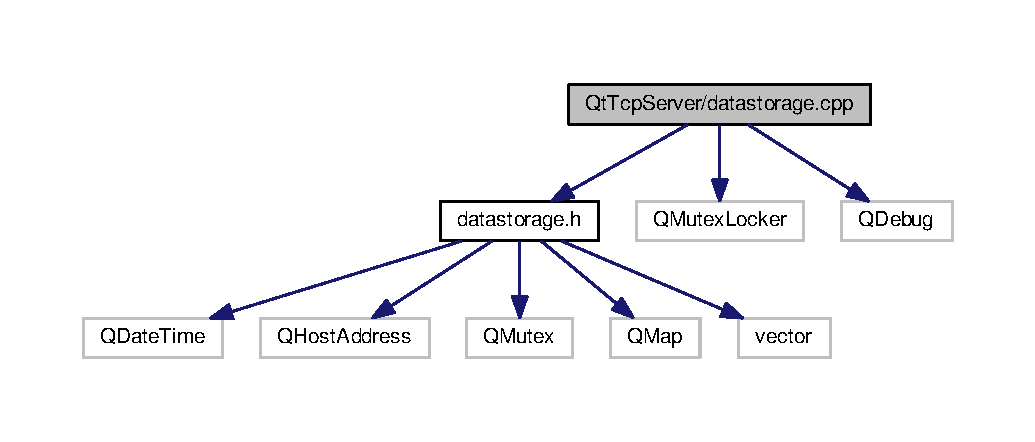
\includegraphics[width=350pt]{datastorage_8cpp__incl}
\end{center}
\end{figure}
\subsection*{Classes}
\begin{DoxyCompactItemize}
\item 
struct \hyperlink{struct_range_test}{Range\+Test}
\end{DoxyCompactItemize}

\hypertarget{datastorage_8h}{}\section{Qt\+Tcp\+Server/datastorage.h File Reference}
\label{datastorage_8h}\index{Qt\+Tcp\+Server/datastorage.\+h@{Qt\+Tcp\+Server/datastorage.\+h}}
{\ttfamily \#include $<$Q\+Date\+Time$>$}\\*
{\ttfamily \#include $<$Q\+Host\+Address$>$}\\*
{\ttfamily \#include $<$Q\+Mutex$>$}\\*
{\ttfamily \#include $<$Q\+Map$>$}\\*
{\ttfamily \#include $<$vector$>$}\\*
Include dependency graph for datastorage.\+h\+:
\nopagebreak
\begin{figure}[H]
\begin{center}
\leavevmode
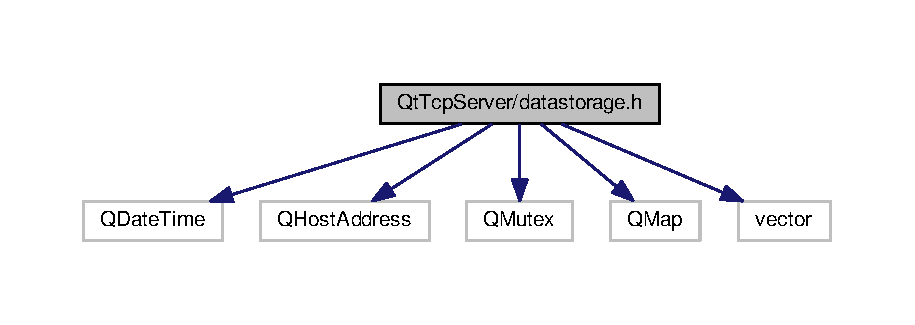
\includegraphics[width=350pt]{datastorage_8h__incl}
\end{center}
\end{figure}
This graph shows which files directly or indirectly include this file\+:
\nopagebreak
\begin{figure}[H]
\begin{center}
\leavevmode
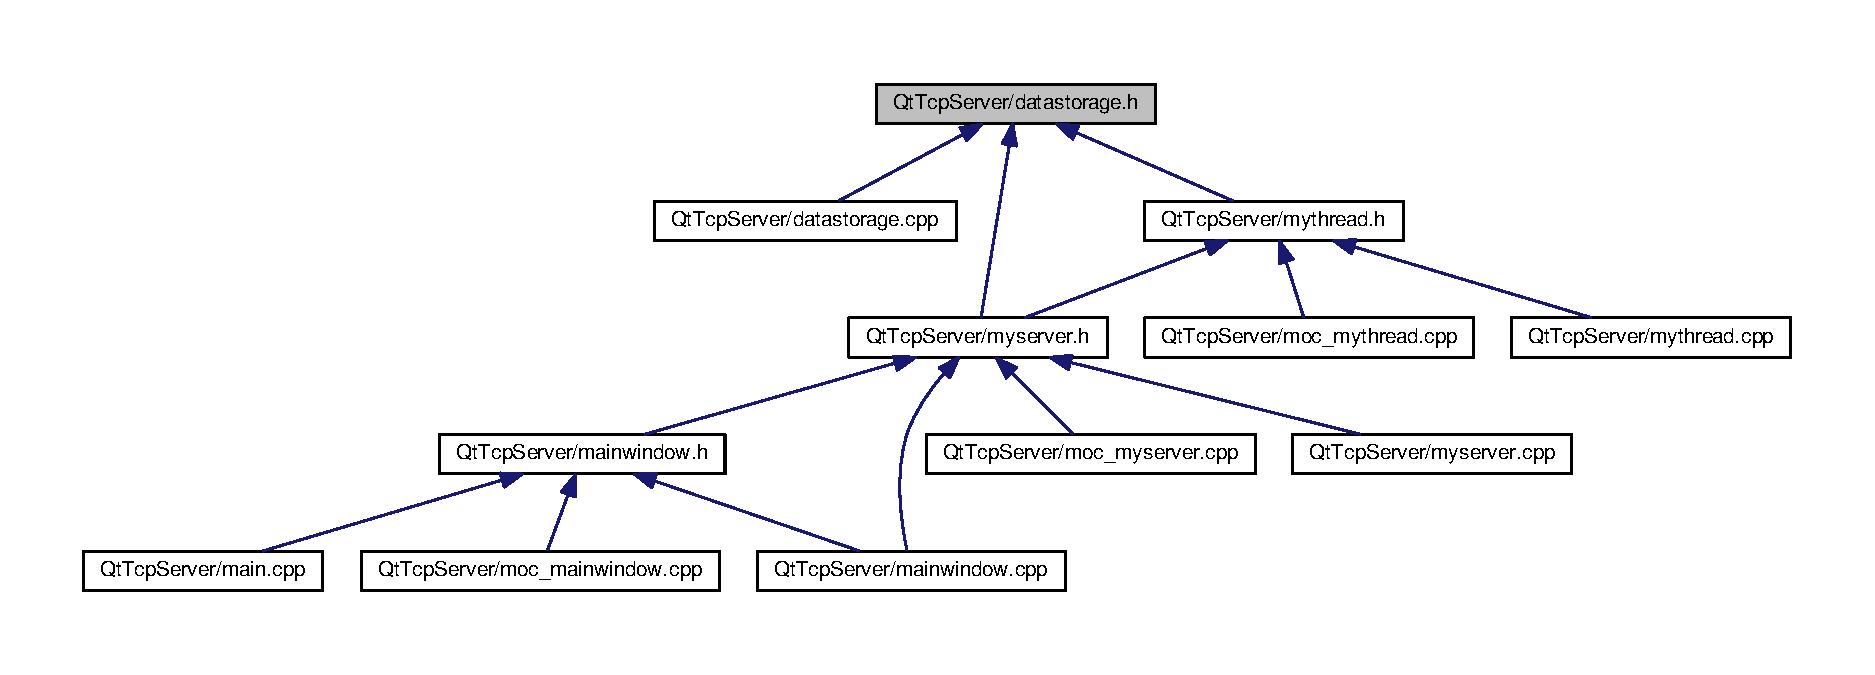
\includegraphics[width=350pt]{datastorage_8h__dep__incl}
\end{center}
\end{figure}
\subsection*{Classes}
\begin{DoxyCompactItemize}
\item 
struct \hyperlink{struct_entry}{Entry}
\item 
class \hyperlink{class_data_storage}{Data\+Storage}
\end{DoxyCompactItemize}

\hypertarget{main_8cpp}{}\section{Referência ao ficheiro main.\+cpp}
\label{main_8cpp}\index{main.\+cpp@{main.\+cpp}}
{\ttfamily \#include \char`\"{}mainwindow.\+h\char`\"{}}\newline
{\ttfamily \#include $<$Q\+Application$>$}\newline
\subsection*{Funções}
\begin{DoxyCompactItemize}
\item 
int \hyperlink{main_8cpp_a0ddf1224851353fc92bfbff6f499fa97}{main} (int argc, char $\ast$argv\mbox{[}$\,$\mbox{]})
\end{DoxyCompactItemize}


\subsection{Documentação das funções}
\mbox{\Hypertarget{main_8cpp_a0ddf1224851353fc92bfbff6f499fa97}\label{main_8cpp_a0ddf1224851353fc92bfbff6f499fa97}} 
\index{main.\+cpp@{main.\+cpp}!main@{main}}
\index{main@{main}!main.\+cpp@{main.\+cpp}}
\subsubsection{\texorpdfstring{main()}{main()}}
{\footnotesize\ttfamily int main (\begin{DoxyParamCaption}\item[{int}]{argc,  }\item[{char $\ast$}]{argv\mbox{[}$\,$\mbox{]} }\end{DoxyParamCaption})}


\hypertarget{mainwindow_8cpp}{}\section{Qt\+Tcp\+Server/mainwindow.cpp File Reference}
\label{mainwindow_8cpp}\index{Qt\+Tcp\+Server/mainwindow.\+cpp@{Qt\+Tcp\+Server/mainwindow.\+cpp}}
{\ttfamily \#include \char`\"{}mainwindow.\+h\char`\"{}}\\*
{\ttfamily \#include \char`\"{}ui\+\_\+mainwindow.\+h\char`\"{}}\\*
{\ttfamily \#include \char`\"{}myserver.\+h\char`\"{}}\\*
{\ttfamily \#include $<$Q\+String\+List$>$}\\*
Include dependency graph for mainwindow.\+cpp\+:
\nopagebreak
\begin{figure}[H]
\begin{center}
\leavevmode
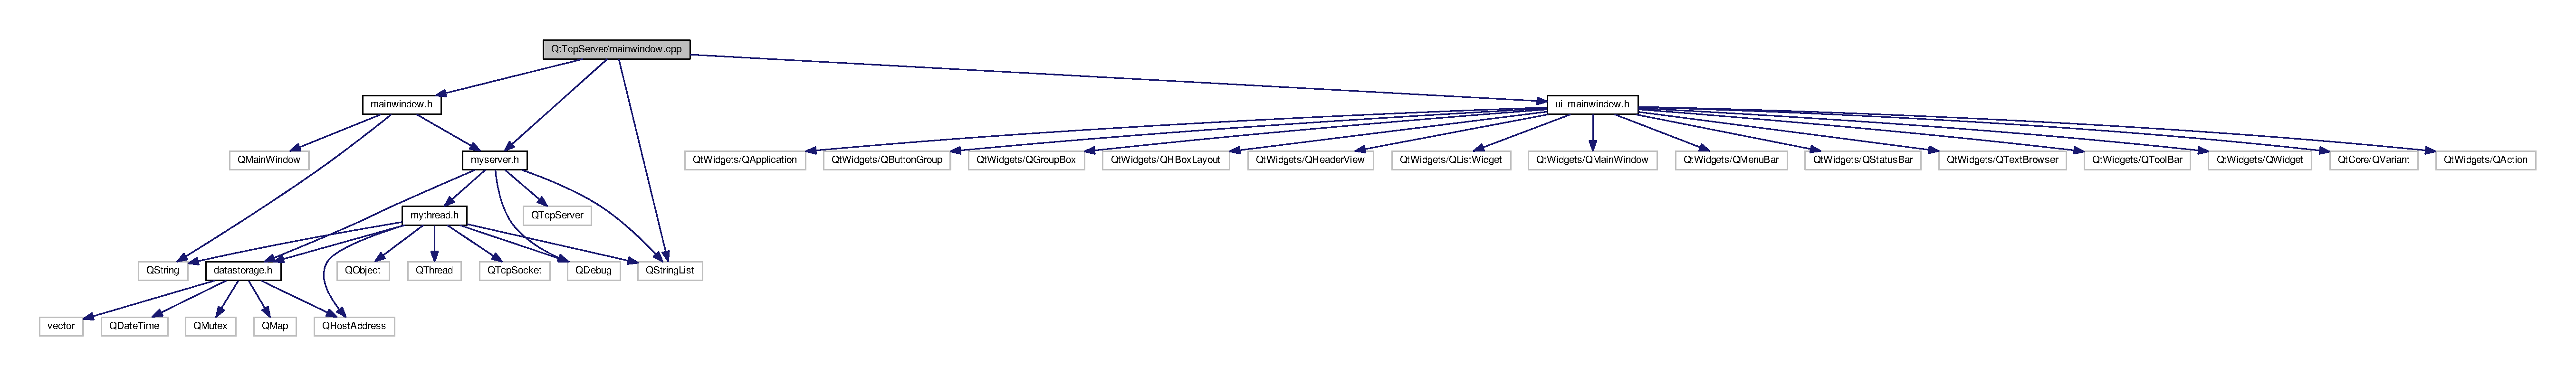
\includegraphics[width=350pt]{mainwindow_8cpp__incl}
\end{center}
\end{figure}

\hypertarget{mainwindow_8h}{}\section{Qt\+Tcp\+Client\+Producer/mainwindow.h File Reference}
\label{mainwindow_8h}\index{Qt\+Tcp\+Client\+Producer/mainwindow.\+h@{Qt\+Tcp\+Client\+Producer/mainwindow.\+h}}
{\ttfamily \#include $<$Q\+Main\+Window$>$}\\*
{\ttfamily \#include $<$Q\+Tcp\+Socket$>$}\\*
{\ttfamily \#include $<$Q\+Debug$>$}\\*
{\ttfamily \#include $<$Q\+String$>$}\\*
Include dependency graph for mainwindow.\+h\+:
\nopagebreak
\begin{figure}[H]
\begin{center}
\leavevmode
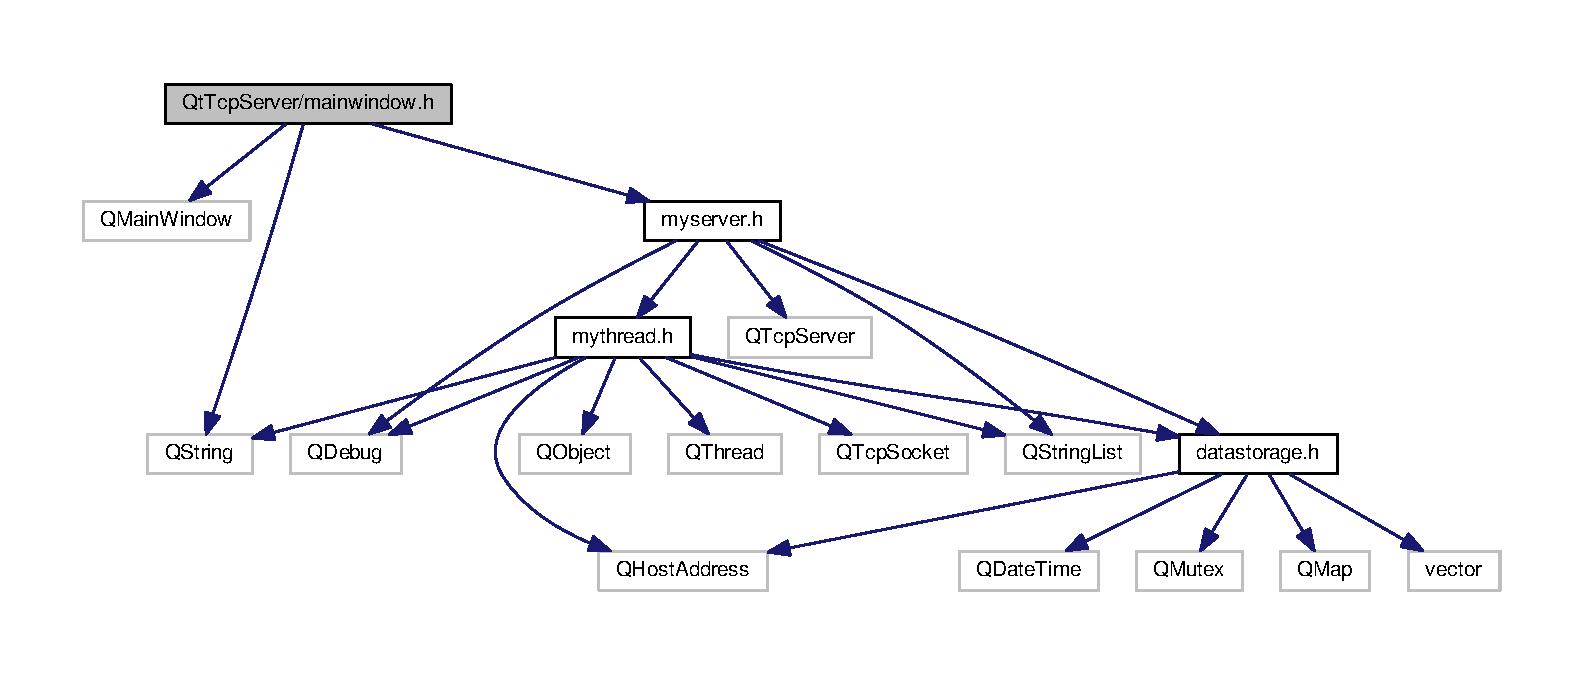
\includegraphics[width=350pt]{mainwindow_8h__incl}
\end{center}
\end{figure}
This graph shows which files directly or indirectly include this file\+:
\nopagebreak
\begin{figure}[H]
\begin{center}
\leavevmode
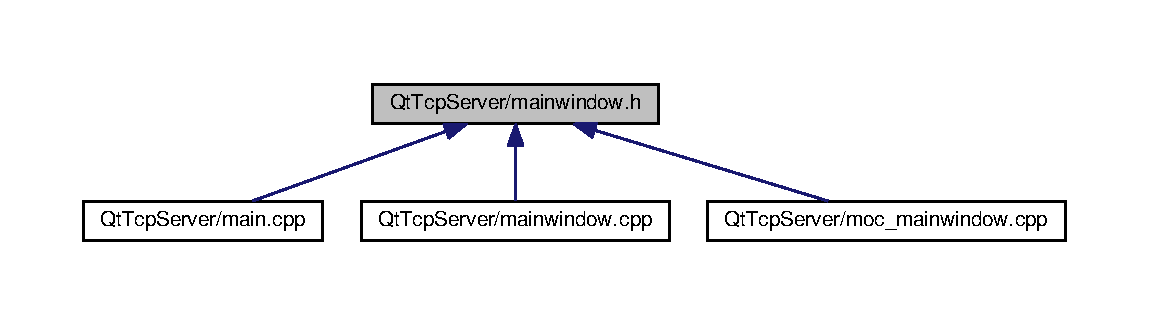
\includegraphics[width=314pt]{mainwindow_8h__dep__incl}
\end{center}
\end{figure}
\subsection*{Classes}
\begin{DoxyCompactItemize}
\item 
class \hyperlink{class_main_window}{Main\+Window}
\begin{DoxyCompactList}\small\item\em A classe \hyperlink{class_main_window}{Main\+Window} representa o contâiner da janela da aplicação e seus componentes. \end{DoxyCompactList}\end{DoxyCompactItemize}
\subsection*{Namespaces}
\begin{DoxyCompactItemize}
\item 
 \hyperlink{namespace_ui}{Ui}
\end{DoxyCompactItemize}

\hypertarget{moc__mainwindow_8cpp}{}\section{Qt\+Tcp\+Server/moc\+\_\+mainwindow.cpp File Reference}
\label{moc__mainwindow_8cpp}\index{Qt\+Tcp\+Server/moc\+\_\+mainwindow.\+cpp@{Qt\+Tcp\+Server/moc\+\_\+mainwindow.\+cpp}}
{\ttfamily \#include \char`\"{}mainwindow.\+h\char`\"{}}\\*
{\ttfamily \#include $<$Qt\+Core/qbytearray.\+h$>$}\\*
{\ttfamily \#include $<$Qt\+Core/qmetatype.\+h$>$}\\*
Include dependency graph for moc\+\_\+mainwindow.\+cpp\+:
\nopagebreak
\begin{figure}[H]
\begin{center}
\leavevmode
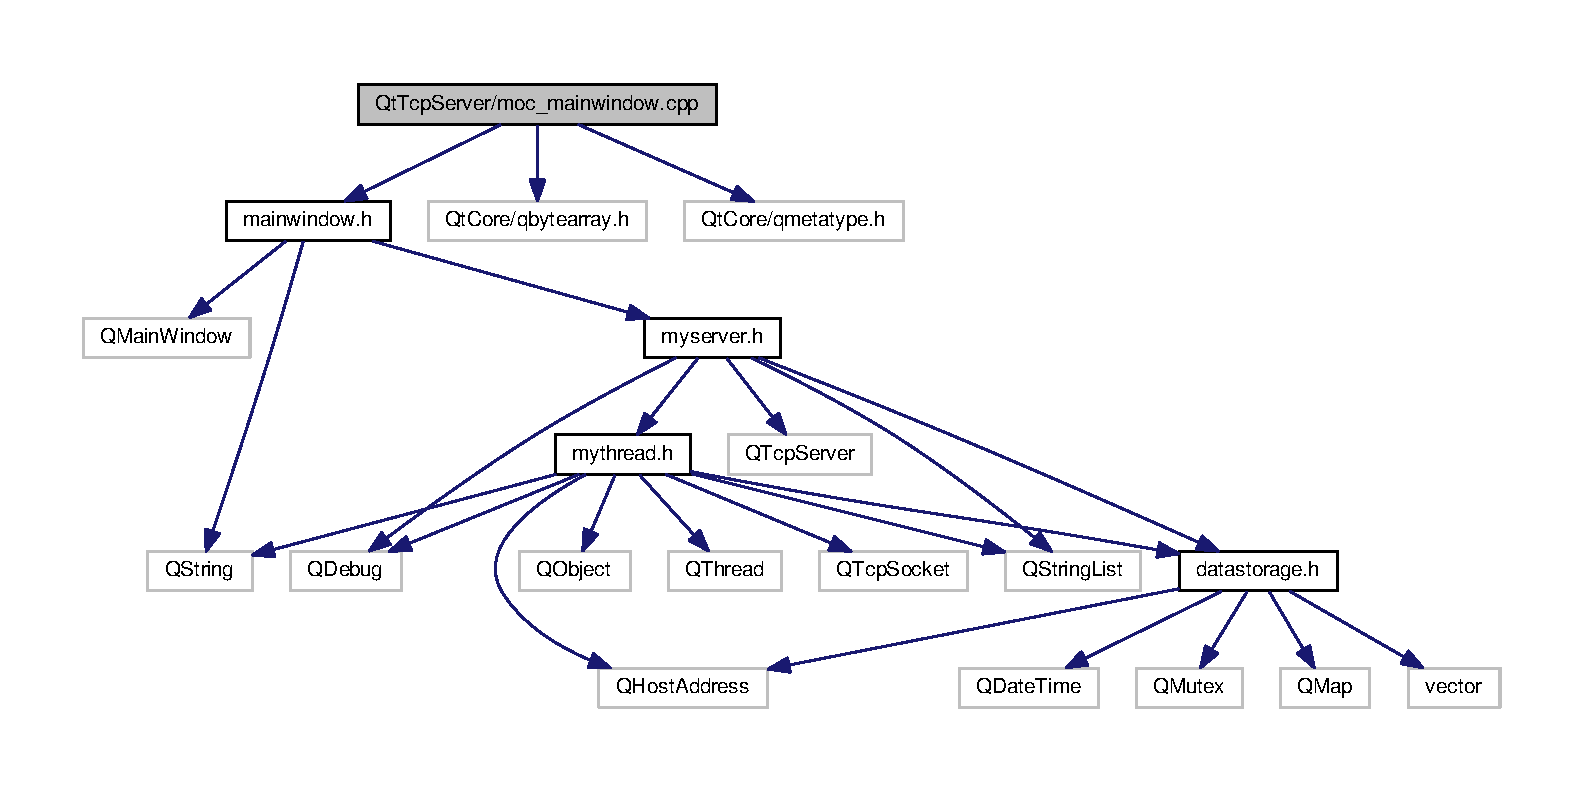
\includegraphics[width=350pt]{moc__mainwindow_8cpp__incl}
\end{center}
\end{figure}
\subsection*{Classes}
\begin{DoxyCompactItemize}
\item 
struct \hyperlink{structqt__meta__stringdata___main_window__t}{qt\+\_\+meta\+\_\+stringdata\+\_\+\+Main\+Window\+\_\+t}
\end{DoxyCompactItemize}
\subsection*{Macros}
\begin{DoxyCompactItemize}
\item 
\#define \hyperlink{moc__mainwindow_8cpp_a75bb9482d242cde0a06c9dbdc6b83abe}{Q\+T\+\_\+\+M\+O\+C\+\_\+\+L\+I\+T\+E\+R\+AL}(idx,  ofs,  len)
\end{DoxyCompactItemize}


\subsection{Macro Definition Documentation}
\index{moc\+\_\+mainwindow.\+cpp@{moc\+\_\+mainwindow.\+cpp}!Q\+T\+\_\+\+M\+O\+C\+\_\+\+L\+I\+T\+E\+R\+AL@{Q\+T\+\_\+\+M\+O\+C\+\_\+\+L\+I\+T\+E\+R\+AL}}
\index{Q\+T\+\_\+\+M\+O\+C\+\_\+\+L\+I\+T\+E\+R\+AL@{Q\+T\+\_\+\+M\+O\+C\+\_\+\+L\+I\+T\+E\+R\+AL}!moc\+\_\+mainwindow.\+cpp@{moc\+\_\+mainwindow.\+cpp}}
\subsubsection[{\texorpdfstring{Q\+T\+\_\+\+M\+O\+C\+\_\+\+L\+I\+T\+E\+R\+AL}{QT_MOC_LITERAL}}]{\setlength{\rightskip}{0pt plus 5cm}\#define Q\+T\+\_\+\+M\+O\+C\+\_\+\+L\+I\+T\+E\+R\+AL(
\begin{DoxyParamCaption}
\item[{}]{idx, }
\item[{}]{ofs, }
\item[{}]{len}
\end{DoxyParamCaption}
)}\hypertarget{moc__mainwindow_8cpp_a75bb9482d242cde0a06c9dbdc6b83abe}{}\label{moc__mainwindow_8cpp_a75bb9482d242cde0a06c9dbdc6b83abe}
{\bfseries Value\+:}
\begin{DoxyCode}
Q\_STATIC\_BYTE\_ARRAY\_DATA\_HEADER\_INITIALIZER\_WITH\_OFFSET(len, \(\backslash\)
    qptrdiff(offsetof(\hyperlink{structqt__meta__stringdata___main_window__t}{qt\_meta\_stringdata\_MainWindow\_t}, stringdata0) + ofs \(\backslash\)
        - idx * \textcolor{keyword}{sizeof}(QByteArrayData)) \(\backslash\)
    )
\end{DoxyCode}

\hypertarget{moc__myserver_8cpp}{}\section{Qt\+Tcp\+Server/moc\+\_\+myserver.cpp File Reference}
\label{moc__myserver_8cpp}\index{Qt\+Tcp\+Server/moc\+\_\+myserver.\+cpp@{Qt\+Tcp\+Server/moc\+\_\+myserver.\+cpp}}
{\ttfamily \#include \char`\"{}myserver.\+h\char`\"{}}\\*
{\ttfamily \#include $<$Qt\+Core/qbytearray.\+h$>$}\\*
{\ttfamily \#include $<$Qt\+Core/qmetatype.\+h$>$}\\*
Include dependency graph for moc\+\_\+myserver.\+cpp\+:
\nopagebreak
\begin{figure}[H]
\begin{center}
\leavevmode
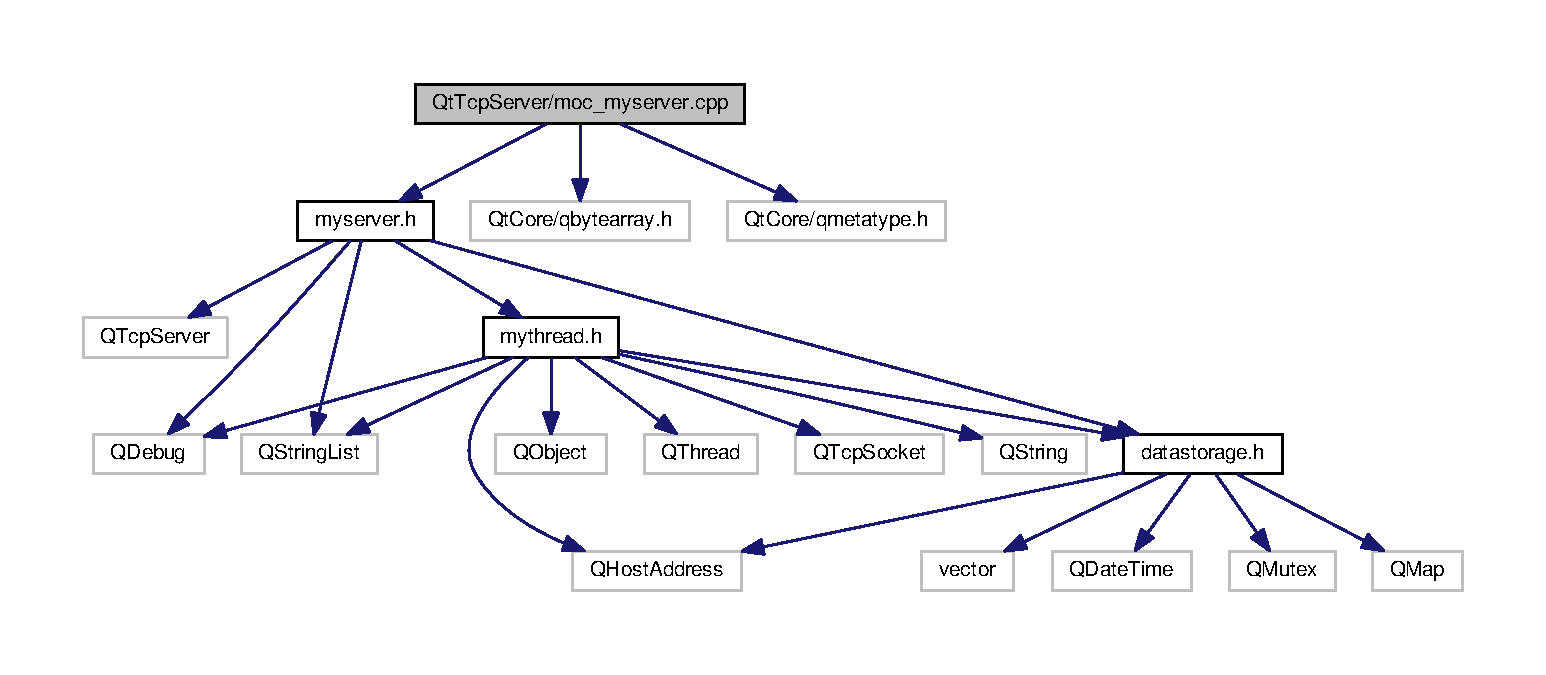
\includegraphics[width=350pt]{moc__myserver_8cpp__incl}
\end{center}
\end{figure}
\subsection*{Classes}
\begin{DoxyCompactItemize}
\item 
struct \hyperlink{structqt__meta__stringdata___my_server__t}{qt\+\_\+meta\+\_\+stringdata\+\_\+\+My\+Server\+\_\+t}
\end{DoxyCompactItemize}
\subsection*{Macros}
\begin{DoxyCompactItemize}
\item 
\#define \hyperlink{moc__myserver_8cpp_a75bb9482d242cde0a06c9dbdc6b83abe}{Q\+T\+\_\+\+M\+O\+C\+\_\+\+L\+I\+T\+E\+R\+AL}(idx,  ofs,  len)
\end{DoxyCompactItemize}


\subsection{Macro Definition Documentation}
\index{moc\+\_\+myserver.\+cpp@{moc\+\_\+myserver.\+cpp}!Q\+T\+\_\+\+M\+O\+C\+\_\+\+L\+I\+T\+E\+R\+AL@{Q\+T\+\_\+\+M\+O\+C\+\_\+\+L\+I\+T\+E\+R\+AL}}
\index{Q\+T\+\_\+\+M\+O\+C\+\_\+\+L\+I\+T\+E\+R\+AL@{Q\+T\+\_\+\+M\+O\+C\+\_\+\+L\+I\+T\+E\+R\+AL}!moc\+\_\+myserver.\+cpp@{moc\+\_\+myserver.\+cpp}}
\subsubsection[{\texorpdfstring{Q\+T\+\_\+\+M\+O\+C\+\_\+\+L\+I\+T\+E\+R\+AL}{QT_MOC_LITERAL}}]{\setlength{\rightskip}{0pt plus 5cm}\#define Q\+T\+\_\+\+M\+O\+C\+\_\+\+L\+I\+T\+E\+R\+AL(
\begin{DoxyParamCaption}
\item[{}]{idx, }
\item[{}]{ofs, }
\item[{}]{len}
\end{DoxyParamCaption}
)}\hypertarget{moc__myserver_8cpp_a75bb9482d242cde0a06c9dbdc6b83abe}{}\label{moc__myserver_8cpp_a75bb9482d242cde0a06c9dbdc6b83abe}
{\bfseries Value\+:}
\begin{DoxyCode}
Q\_STATIC\_BYTE\_ARRAY\_DATA\_HEADER\_INITIALIZER\_WITH\_OFFSET(len, \(\backslash\)
    qptrdiff(offsetof(\hyperlink{structqt__meta__stringdata___my_server__t}{qt\_meta\_stringdata\_MyServer\_t}, stringdata0) + ofs \(\backslash\)
        - idx * \textcolor{keyword}{sizeof}(QByteArrayData)) \(\backslash\)
    )
\end{DoxyCode}

\hypertarget{moc__mythread_8cpp}{}\section{Qt\+Tcp\+Server/moc\+\_\+mythread.cpp File Reference}
\label{moc__mythread_8cpp}\index{Qt\+Tcp\+Server/moc\+\_\+mythread.\+cpp@{Qt\+Tcp\+Server/moc\+\_\+mythread.\+cpp}}
{\ttfamily \#include \char`\"{}mythread.\+h\char`\"{}}\\*
{\ttfamily \#include $<$Qt\+Core/qbytearray.\+h$>$}\\*
{\ttfamily \#include $<$Qt\+Core/qmetatype.\+h$>$}\\*
Include dependency graph for moc\+\_\+mythread.\+cpp\+:
\nopagebreak
\begin{figure}[H]
\begin{center}
\leavevmode
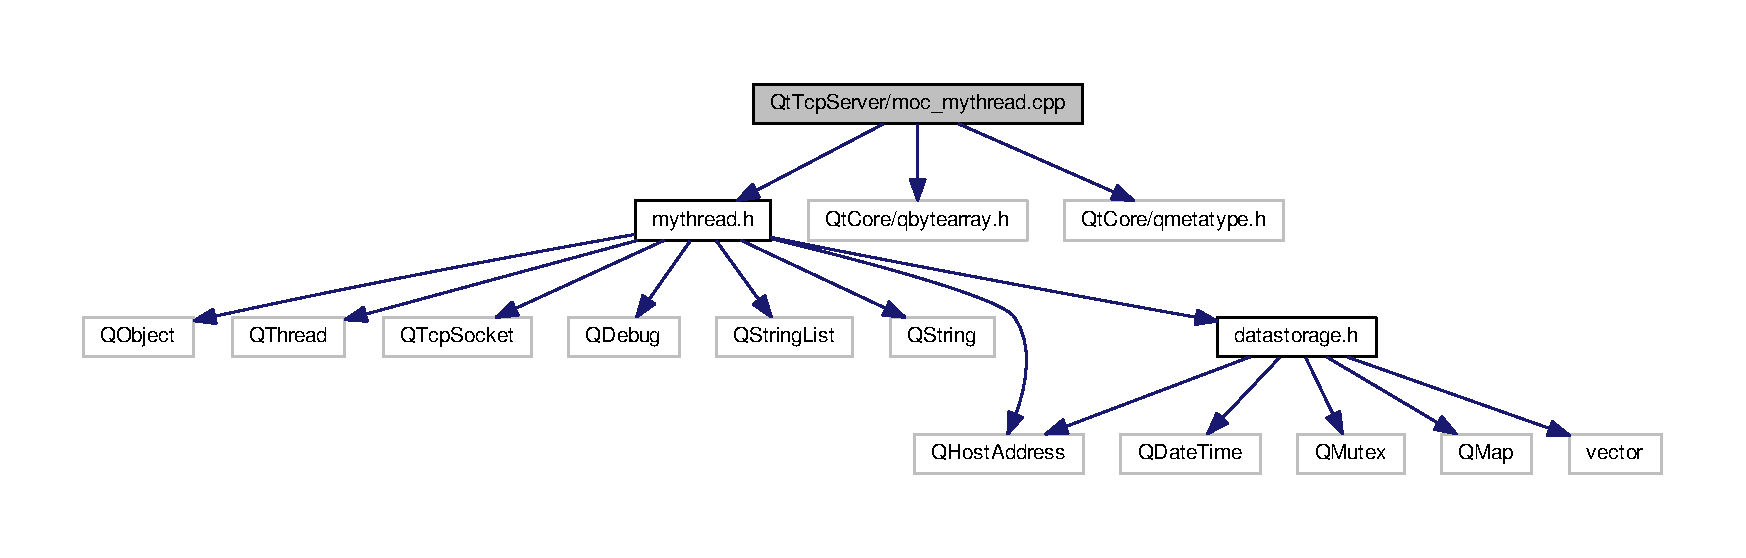
\includegraphics[width=350pt]{moc__mythread_8cpp__incl}
\end{center}
\end{figure}
\subsection*{Classes}
\begin{DoxyCompactItemize}
\item 
struct \hyperlink{structqt__meta__stringdata___my_thread__t}{qt\+\_\+meta\+\_\+stringdata\+\_\+\+My\+Thread\+\_\+t}
\end{DoxyCompactItemize}
\subsection*{Macros}
\begin{DoxyCompactItemize}
\item 
\#define \hyperlink{moc__mythread_8cpp_a75bb9482d242cde0a06c9dbdc6b83abe}{Q\+T\+\_\+\+M\+O\+C\+\_\+\+L\+I\+T\+E\+R\+AL}(idx,  ofs,  len)
\end{DoxyCompactItemize}


\subsection{Macro Definition Documentation}
\index{moc\+\_\+mythread.\+cpp@{moc\+\_\+mythread.\+cpp}!Q\+T\+\_\+\+M\+O\+C\+\_\+\+L\+I\+T\+E\+R\+AL@{Q\+T\+\_\+\+M\+O\+C\+\_\+\+L\+I\+T\+E\+R\+AL}}
\index{Q\+T\+\_\+\+M\+O\+C\+\_\+\+L\+I\+T\+E\+R\+AL@{Q\+T\+\_\+\+M\+O\+C\+\_\+\+L\+I\+T\+E\+R\+AL}!moc\+\_\+mythread.\+cpp@{moc\+\_\+mythread.\+cpp}}
\subsubsection[{\texorpdfstring{Q\+T\+\_\+\+M\+O\+C\+\_\+\+L\+I\+T\+E\+R\+AL}{QT_MOC_LITERAL}}]{\setlength{\rightskip}{0pt plus 5cm}\#define Q\+T\+\_\+\+M\+O\+C\+\_\+\+L\+I\+T\+E\+R\+AL(
\begin{DoxyParamCaption}
\item[{}]{idx, }
\item[{}]{ofs, }
\item[{}]{len}
\end{DoxyParamCaption}
)}\hypertarget{moc__mythread_8cpp_a75bb9482d242cde0a06c9dbdc6b83abe}{}\label{moc__mythread_8cpp_a75bb9482d242cde0a06c9dbdc6b83abe}
{\bfseries Value\+:}
\begin{DoxyCode}
Q\_STATIC\_BYTE\_ARRAY\_DATA\_HEADER\_INITIALIZER\_WITH\_OFFSET(len, \(\backslash\)
    qptrdiff(offsetof(\hyperlink{structqt__meta__stringdata___my_thread__t}{qt\_meta\_stringdata\_MyThread\_t}, stringdata0) + ofs \(\backslash\)
        - idx * \textcolor{keyword}{sizeof}(QByteArrayData)) \(\backslash\)
    )
\end{DoxyCode}

\hypertarget{myserver_8cpp}{}\section{Qt\+Tcp\+Server/myserver.cpp File Reference}
\label{myserver_8cpp}\index{Qt\+Tcp\+Server/myserver.\+cpp@{Qt\+Tcp\+Server/myserver.\+cpp}}
{\ttfamily \#include \char`\"{}myserver.\+h\char`\"{}}\\*
{\ttfamily \#include $<$Q\+Network\+Interface$>$}\\*
Include dependency graph for myserver.\+cpp\+:
\nopagebreak
\begin{figure}[H]
\begin{center}
\leavevmode
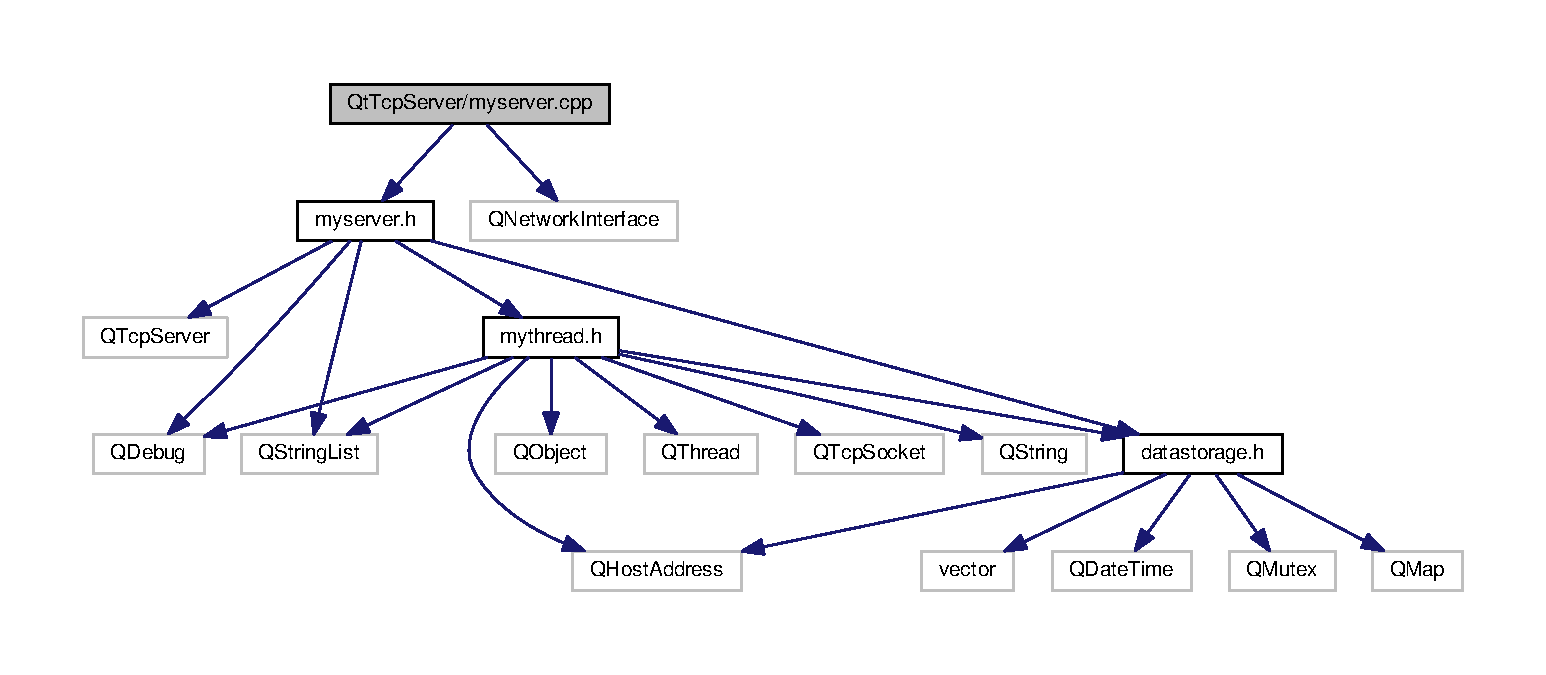
\includegraphics[width=350pt]{myserver_8cpp__incl}
\end{center}
\end{figure}

\hypertarget{myserver_8h}{}\section{Qt\+Tcp\+Server/myserver.h File Reference}
\label{myserver_8h}\index{Qt\+Tcp\+Server/myserver.\+h@{Qt\+Tcp\+Server/myserver.\+h}}
{\ttfamily \#include $<$Q\+Tcp\+Server$>$}\\*
{\ttfamily \#include $<$Q\+Debug$>$}\\*
{\ttfamily \#include $<$Q\+String\+List$>$}\\*
{\ttfamily \#include \char`\"{}mythread.\+h\char`\"{}}\\*
{\ttfamily \#include \char`\"{}datastorage.\+h\char`\"{}}\\*
Include dependency graph for myserver.\+h\+:
\nopagebreak
\begin{figure}[H]
\begin{center}
\leavevmode
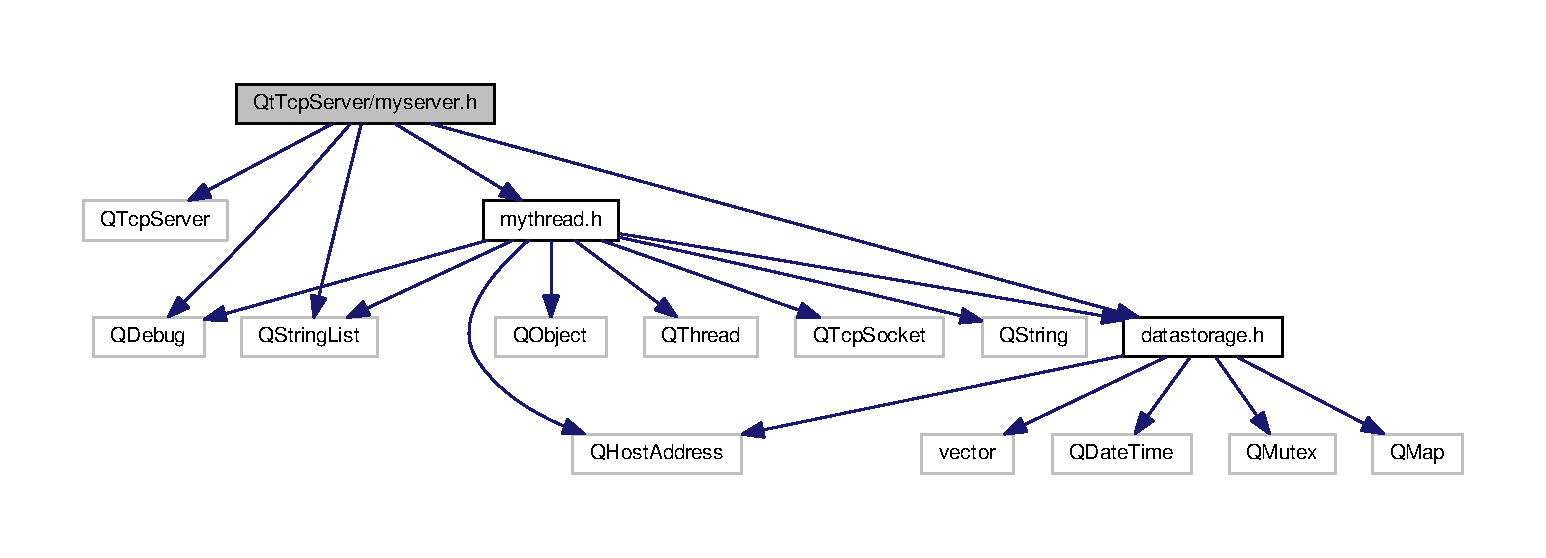
\includegraphics[width=350pt]{myserver_8h__incl}
\end{center}
\end{figure}
This graph shows which files directly or indirectly include this file\+:
\nopagebreak
\begin{figure}[H]
\begin{center}
\leavevmode
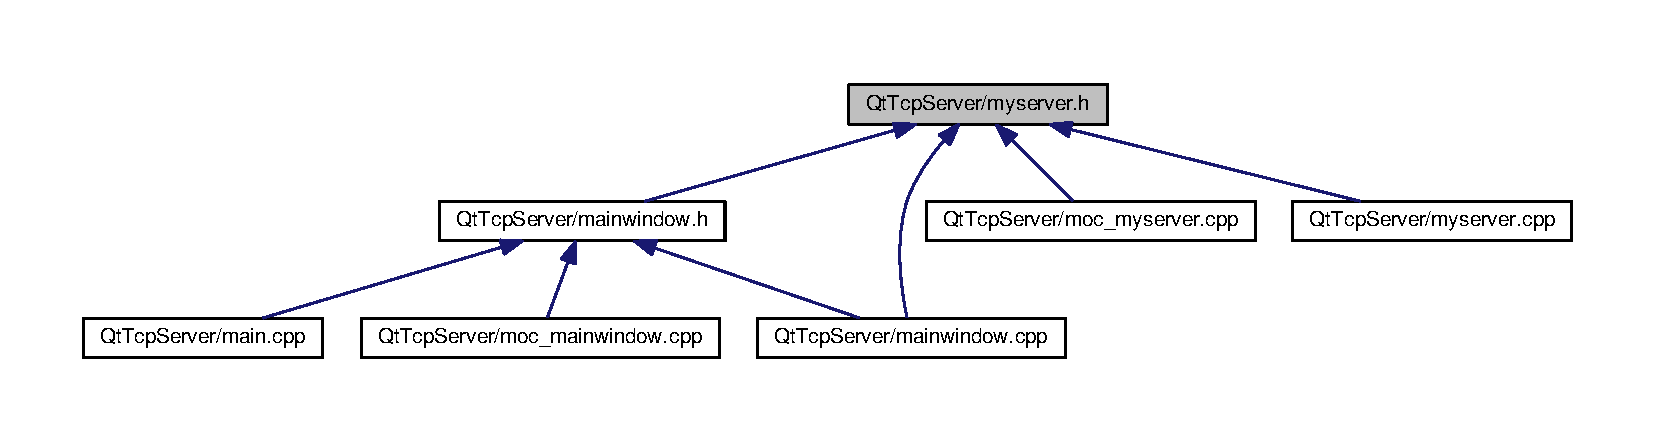
\includegraphics[width=350pt]{myserver_8h__dep__incl}
\end{center}
\end{figure}
\subsection*{Classes}
\begin{DoxyCompactItemize}
\item 
class \hyperlink{class_my_server}{My\+Server}
\begin{DoxyCompactList}\small\item\em The \hyperlink{class_my_server}{My\+Server} class inicia um servidor T\+CP capaz de \char`\"{}ouvir\char`\"{} a porta 1234. \end{DoxyCompactList}\end{DoxyCompactItemize}

\hypertarget{mythread_8cpp}{}\section{Qt\+Tcp\+Server/mythread.cpp File Reference}
\label{mythread_8cpp}\index{Qt\+Tcp\+Server/mythread.\+cpp@{Qt\+Tcp\+Server/mythread.\+cpp}}
{\ttfamily \#include \char`\"{}mythread.\+h\char`\"{}}\\*
{\ttfamily \#include $<$vector$>$}\\*
Include dependency graph for mythread.\+cpp\+:
\nopagebreak
\begin{figure}[H]
\begin{center}
\leavevmode
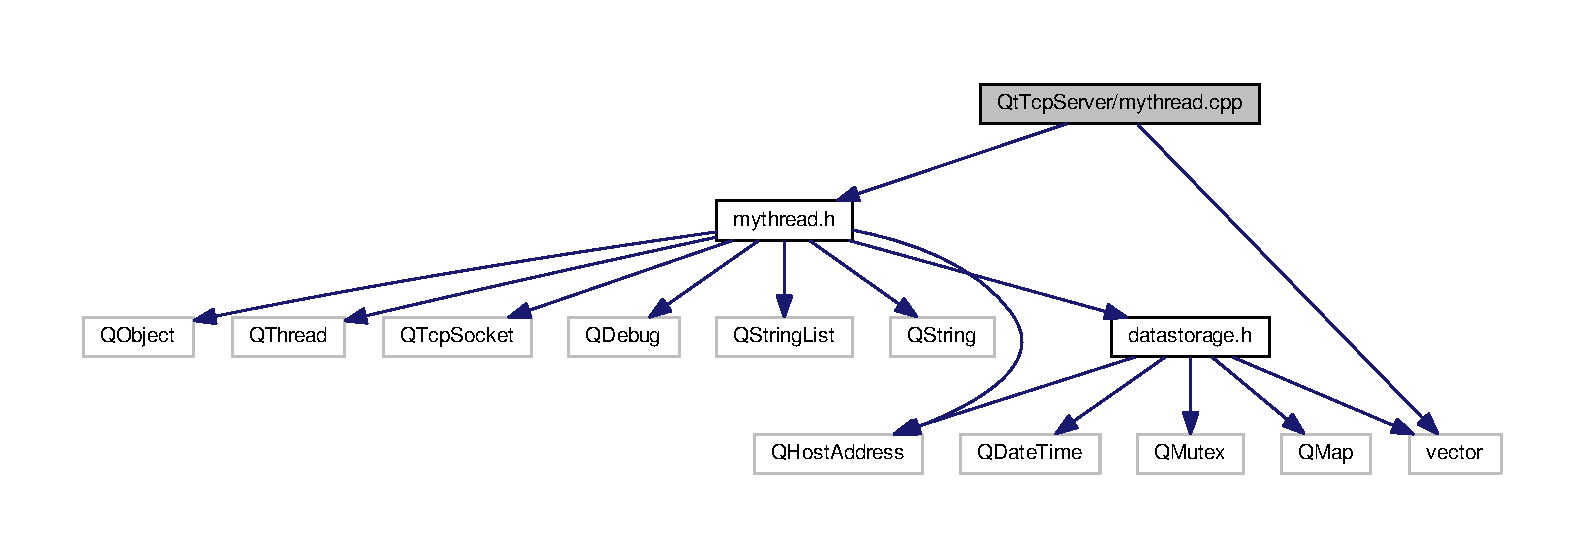
\includegraphics[width=350pt]{mythread_8cpp__incl}
\end{center}
\end{figure}

\hypertarget{mythread_8h}{}\section{Qt\+Tcp\+Server/mythread.h File Reference}
\label{mythread_8h}\index{Qt\+Tcp\+Server/mythread.\+h@{Qt\+Tcp\+Server/mythread.\+h}}
{\ttfamily \#include $<$Q\+Object$>$}\\*
{\ttfamily \#include $<$Q\+Thread$>$}\\*
{\ttfamily \#include $<$Q\+Tcp\+Socket$>$}\\*
{\ttfamily \#include $<$Q\+Debug$>$}\\*
{\ttfamily \#include $<$Q\+String\+List$>$}\\*
{\ttfamily \#include $<$Q\+String$>$}\\*
{\ttfamily \#include $<$Q\+Host\+Address$>$}\\*
{\ttfamily \#include \char`\"{}datastorage.\+h\char`\"{}}\\*
Include dependency graph for mythread.\+h\+:
\nopagebreak
\begin{figure}[H]
\begin{center}
\leavevmode
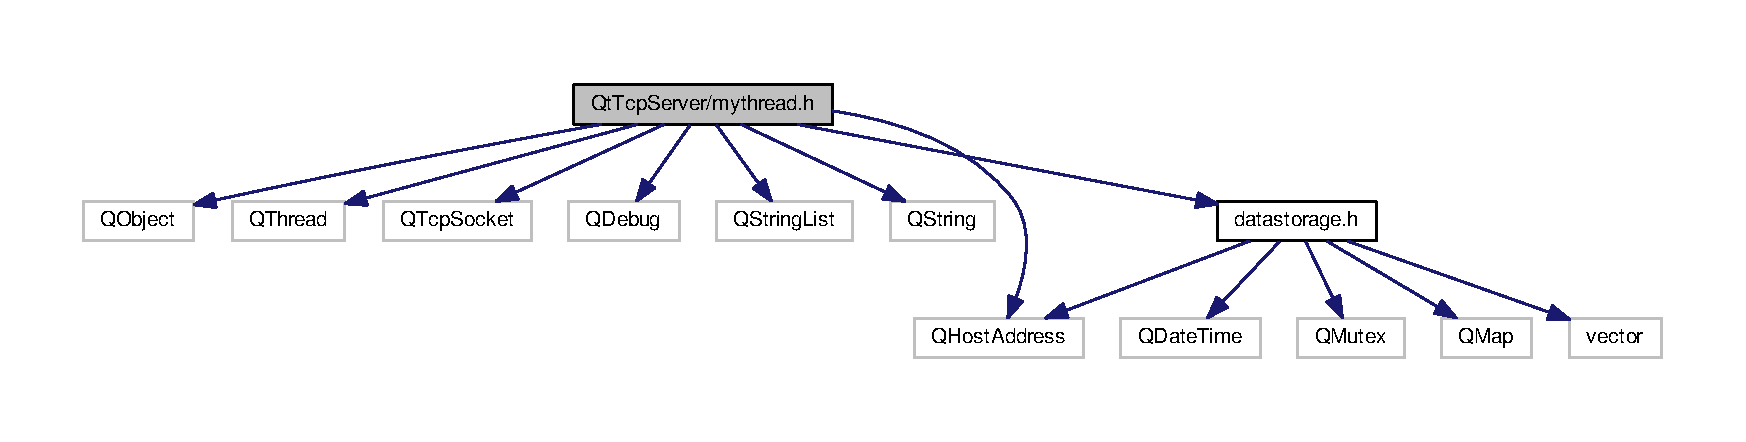
\includegraphics[width=350pt]{mythread_8h__incl}
\end{center}
\end{figure}
This graph shows which files directly or indirectly include this file\+:
\nopagebreak
\begin{figure}[H]
\begin{center}
\leavevmode
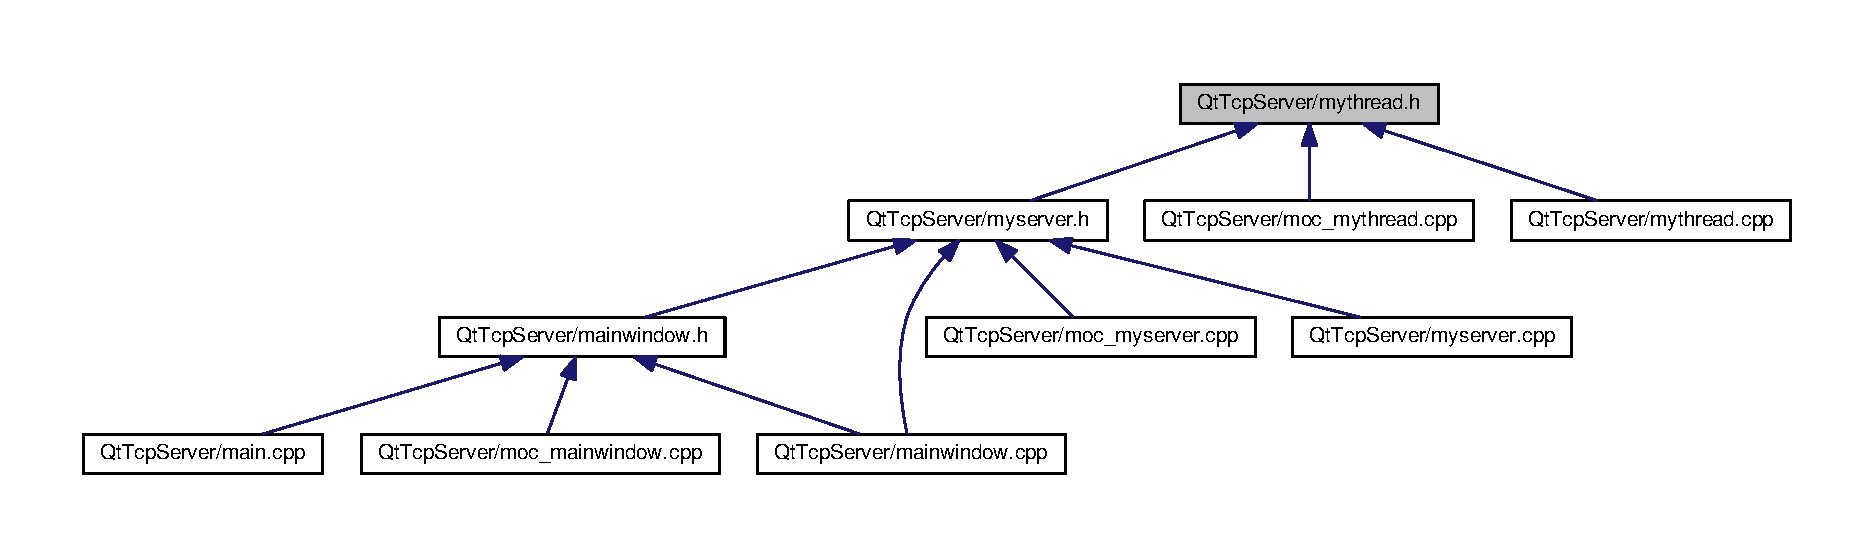
\includegraphics[width=350pt]{mythread_8h__dep__incl}
\end{center}
\end{figure}
\subsection*{Classes}
\begin{DoxyCompactItemize}
\item 
class \hyperlink{class_my_thread}{My\+Thread}
\begin{DoxyCompactList}\small\item\em The \hyperlink{class_my_thread}{My\+Thread} class cria uma thread que lida com o tratamento de uma conexao T\+CP de entrada. \end{DoxyCompactList}\end{DoxyCompactItemize}

\hypertarget{ui__mainwindow_8h}{}\section{Qt\+Tcp\+Server/ui\+\_\+mainwindow.h File Reference}
\label{ui__mainwindow_8h}\index{Qt\+Tcp\+Server/ui\+\_\+mainwindow.\+h@{Qt\+Tcp\+Server/ui\+\_\+mainwindow.\+h}}
{\ttfamily \#include $<$Qt\+Core/\+Q\+Variant$>$}\\*
{\ttfamily \#include $<$Qt\+Widgets/\+Q\+Action$>$}\\*
{\ttfamily \#include $<$Qt\+Widgets/\+Q\+Application$>$}\\*
{\ttfamily \#include $<$Qt\+Widgets/\+Q\+Button\+Group$>$}\\*
{\ttfamily \#include $<$Qt\+Widgets/\+Q\+Group\+Box$>$}\\*
{\ttfamily \#include $<$Qt\+Widgets/\+Q\+H\+Box\+Layout$>$}\\*
{\ttfamily \#include $<$Qt\+Widgets/\+Q\+Header\+View$>$}\\*
{\ttfamily \#include $<$Qt\+Widgets/\+Q\+List\+Widget$>$}\\*
{\ttfamily \#include $<$Qt\+Widgets/\+Q\+Main\+Window$>$}\\*
{\ttfamily \#include $<$Qt\+Widgets/\+Q\+Menu\+Bar$>$}\\*
{\ttfamily \#include $<$Qt\+Widgets/\+Q\+Status\+Bar$>$}\\*
{\ttfamily \#include $<$Qt\+Widgets/\+Q\+Text\+Browser$>$}\\*
{\ttfamily \#include $<$Qt\+Widgets/\+Q\+Tool\+Bar$>$}\\*
{\ttfamily \#include $<$Qt\+Widgets/\+Q\+Widget$>$}\\*
Include dependency graph for ui\+\_\+mainwindow.\+h\+:
\nopagebreak
\begin{figure}[H]
\begin{center}
\leavevmode
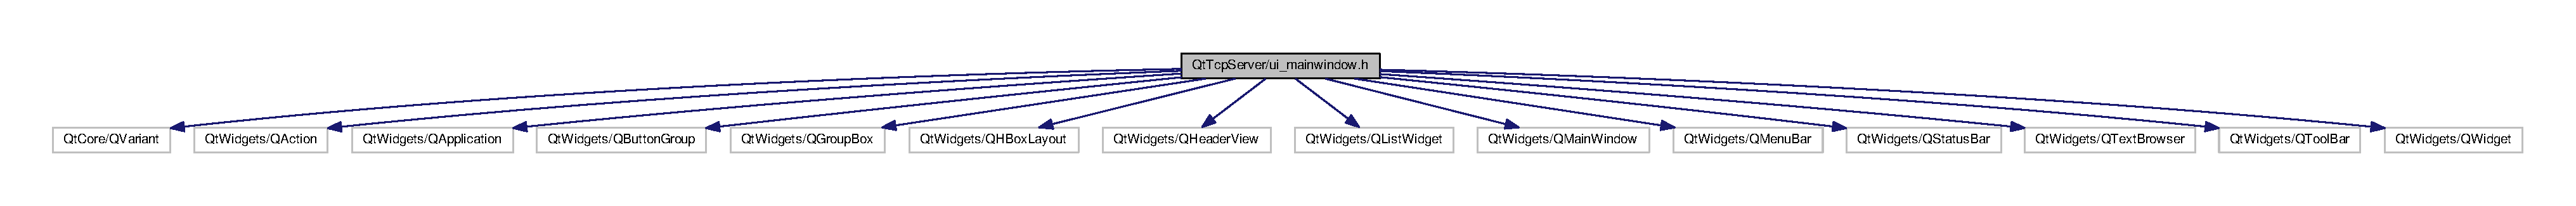
\includegraphics[width=350pt]{ui__mainwindow_8h__incl}
\end{center}
\end{figure}
This graph shows which files directly or indirectly include this file\+:
\nopagebreak
\begin{figure}[H]
\begin{center}
\leavevmode
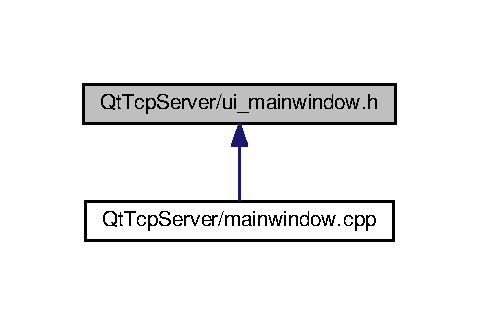
\includegraphics[width=230pt]{ui__mainwindow_8h__dep__incl}
\end{center}
\end{figure}
\subsection*{Classes}
\begin{DoxyCompactItemize}
\item 
class \hyperlink{class_ui___main_window}{Ui\+\_\+\+Main\+Window}
\item 
class \hyperlink{class_ui_1_1_main_window}{Ui\+::\+Main\+Window}
\end{DoxyCompactItemize}
\subsection*{Namespaces}
\begin{DoxyCompactItemize}
\item 
 \hyperlink{namespace_ui}{Ui}
\end{DoxyCompactItemize}

%--- End generated contents ---

% Index
\backmatter
\newpage
\phantomsection
\clearemptydoublepage
\addcontentsline{toc}{chapter}{Index}
\printindex

\end{document}
